\chapter{Results} \label{chap:results} % 20-30 pages

This chapter presents and discusses the evaluation of the proposed anomaly detection approach for video. As described in the previous chapter, evaluation of the anomaly detection system (ADS) is done by first training the video generation model for next-frame prediction, before that model is loaded into IFTM (see Section \ref{sec:framework}). The resulting ADS is then run on a labeled evaluation video data set. Evaluation of the two components is decoupled at first: In Section \ref{sec:cvgan_eval}, the evaluation method and the results for the video prediction model are presented. Then in Section \ref{sec:vad_eval}, the quality of the IFTM ADS using the already evaluated prediction models is assessed. Finally in Section \ref{sec:discussion}, both results are discussed and linked to each other.

Evaluation was performed on a workstation running Windows 10 with 32 GB RAM, a 4.2 GHz Intel i7 quad-core processor, and a Nvidia GeForce 3090 graphics card with 24 GB VRAM. A full evaluation run of a single hyperparameter configuration usually took 24--48 hours depending on the configuration and the load of the system. An implementation of the analysis framework is available online\footnote{\url{https://github.com/fshofmann/video-anomaly-detection}}.



% C-VGAN Evaluation
\section{C-GAN for Video Forecasting} \label{sec:cvgan_eval}

For the evaluation of video generation models, the focus in this work lies solely on our modified version of C-VGAN presented in Section \ref{subsec:vgan_mod_2} and not on any of the preceding versions. As explained in Section \ref{subsec:framework_cvgan}, our framework saves any models during and after training to disk, to allow them to be used for anomaly detection evaluation. To find optimal prediction models for this task, these models need to be evaluated on their own without direct connection to the task of video anomaly detection (VAD). However it is unfeasible to evaluate many hyperparameter configurations due to the high number of trainable parameters in the two models, that need to be optimized until a convergence of losses of the two adversarial models is achieved (see Section \ref{sec:gans}). Therefore as explained in the presentation of the framework, the number of non-fixed hyperparameters is heavily limited and their initial values are based on configurations of DCGAN \cite{radford2015unsupervised}, VGAN, and C-VGAN \cite{vondrick2016generating}. Training of each configuration is fixed to 50 epochs, since most models maintained their loss-equilibrium till that number of training iterations.

The performance of all configurations is evaluated based on quantitative evaluation metrics but also on qualitative ones, i.e. visual, assessment. The reasoning behind that will be explained in the following section, while further insight into these metrics will be provided as well. Afterwards the results for our models using different hyperparameter configurations are presented. This includes additional information on the tuning of thereof.


% C-VGAN Evaluation Methods
\subsection{Evaluation Method} \label{subsec:cvgan_eval_method} % 3 Pages

\paragraph{Hold-Out Validation}
First, to evaluate a model on its ability to predict the next frame from a fixed set of past frames, the quality of the model cannot be assessed using observations with which the model was trained. Worst case, models are able to accurately reflect the training observations and thus make perfect predictions for them, while being unable to work with unknown inputs at runtime. However at the same time, the evaluation data set presented in Section \ref{sec:dataset}, is not helpful to evaluate the quality of a next-frame prediction model. At least from a generalization perspective: As this data set tries to disrupt the prediction model by giving it both normal and anomalous videos, the model must be unable to model these anomalous properties found in that data set and make predictions that differ to the actual videos. Therefore a good generalization performance on that data set would cause an equally bad anomaly detection performance, as IFTM would be unable to differentiate between the predictions errors of normal and anomalous observations.  

\begin{figure}
	\centering
	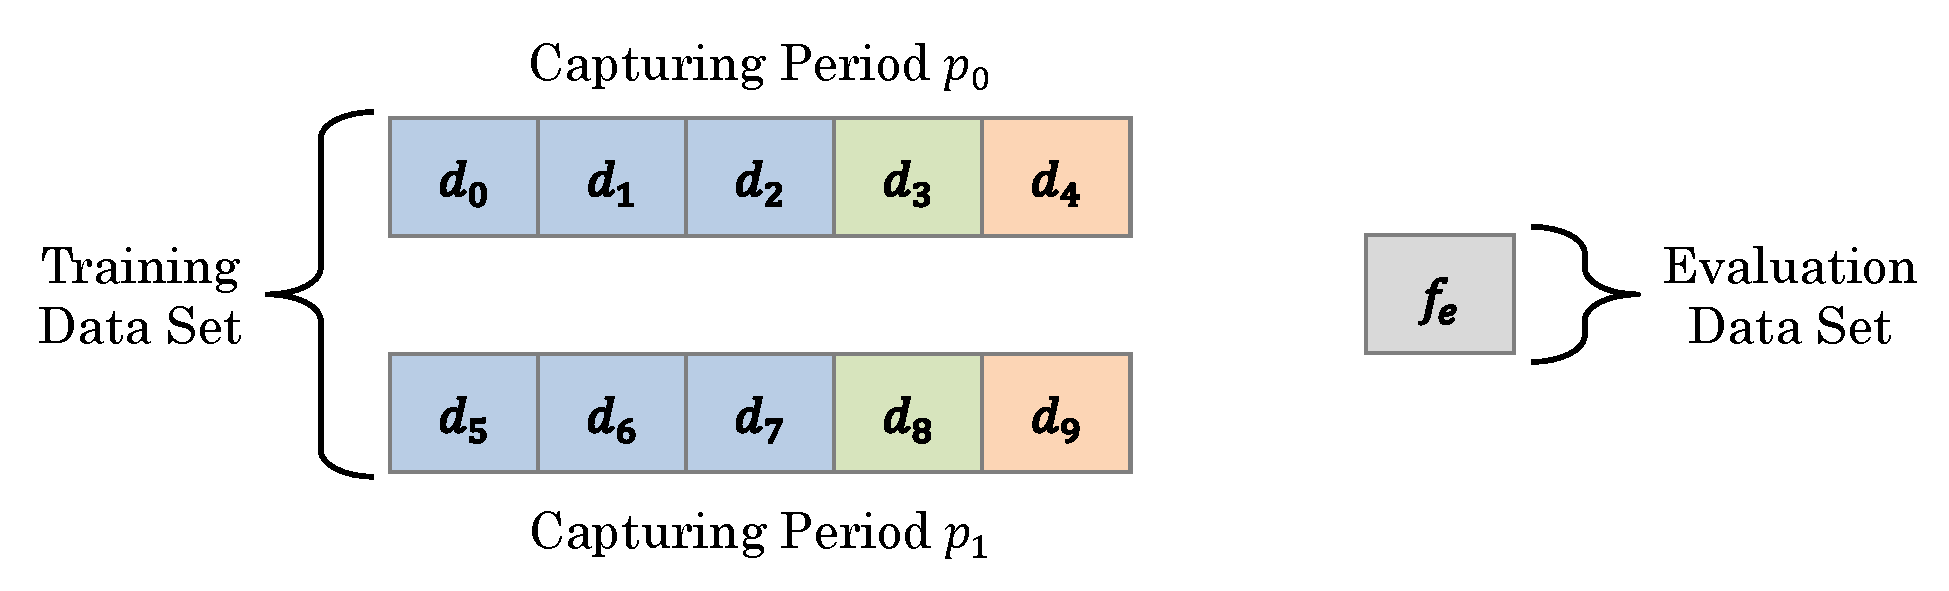
\includegraphics[width=0.9\textwidth]{graphics/eval/evalSplit/evalSplit.pdf}
  \caption[Splitting of the data set for evaluation.]{Splitting of the data set into training (blue), validation (green), and test set (orange). The evaluation data set (gray) is used at a later stage and relevant for the prediction model's qualitative evaluation.}
  \label{fig:dataset_split}
\end{figure}

Thus the training data set consisting of $10$ days is further split into three parts, as illustrated in Figure \ref{fig:dataset_split}. Six days, three from each capturing period (see Section \ref{sec:dataset}), will be given to the model during training. Then, the model's quality is validated after the completion of every training epoch using two other days of video material. Lastly, the remaining two days are chosen as the test set to measure the quality of the final model independently from the tuning of the hyperparameters. This kind of hold-out validation with fixed subsets is to be preferred over exhaustive cross-validation methods in which all combinations of subsets are used to train, validate, and test the model iteratively, before the respective errors across runs are averaged \cite{stone1974cross}. The long time to fully train a single model configuration --- up to $48$ hours, makes the latter methods unfeasible for this work, as they would greatly reduce the number of different hyperparameter configurations one can explore and evaluate. 

\paragraph{Model Losses}
Training, validating, and testing the model require the measuring of the models' value function, that is optimized during training. As GANs consist of two models that play a min-max game to optimize said function, as explained in Section \ref{sec:gans}, one can take said function and disassemble it into the loss terms that are minimized by each of the two models. Applying this to the adapted value function of C-VGAN for next-frame prediction from Section \ref{par:vgan_mod_2_vfn}, this results in the following loss functions for the generator $G$ and discriminator $D$, respectively:

\begin{equation} \label{eq:loss_g}
\mathcal{L}_G = \mathbb{E}_{x_{0;6} \sim p_{x_{0;6}}(x_{0;6})}[\log(1 - D(G(x_{0;6})))] + \mathbb{E}_{x_{0;6} \sim p_{x_{0;6}}(x_{0;6})}[\lambda \cdot \|(x_{0;6} - G^{0;6}(x_{0;6}))\|_1]
\end{equation}

\begin{equation} \label{eq:loss_d}
\mathcal{L}_D = - \mathbb{E}_{x \sim p_x(x)}[\log D(x)] - \mathbb{E}_{x_{0;6} \sim p_{x_{0;6}}(x_{0;6})}[\log(1 - D(G(x_{0;6})))]
\end{equation}

During training, these losses are computed batch wise, i.e. for each training step in an epoch, and the average of thereof is computed at the end of every epoch for evaluation purposes: Disregarding the reconstruction loss (second loss term of $\mathcal{L}_G$), training of the two models is a zero-sum game in which both models' losses should converge to non-zero values over the epochs, as they improve in parallel. Failure to converge is a sufficient indicator for a failure mode in training and a high certainty that the models are of poor quality; see Section \ref{par:failure_modes} and the paragraph about the common failure models in GAN training. In addition, after the completion of every epoch, the models are validated using the validation split of the data set and the models' validation losses are computed and recorded as well. The same is done with the test data set after the entire training procedure is completed. It is to note, that validation and test losses are only of use if failure to generalize is one-sided and does not affect both models, as the loss functions influence each other. But even if the latter occurs, differences in the losses' behavior during training can be of interest. For example it would be ideal if both training and validation losses converged in similar manner. Any fluctuations of the validation losses while training losses were stable would be an indicator for overfitting models that are not able to generalize well. Finally, the generator loss also serves as a strong indicator whether the generator is even able to reconstruct past frames, as, depending on the choice for $\lambda$, the reconstruction term is dominating the generator's loss function.

\paragraph{Qualitative Evaluation} \label{par:cvgan_eval_method_qual}
While failure modes in the training of GANs are most of the time an indicator that something has gone wrong and the models have to be discarded, a successful convergence of the losses does not imply the GANs have successfully completed training: Failure to model certain motion dynamics, hallucinating or the omission of objects, or simply the generation unrealistic looking videos can still occur. This happens sometimes when either the capacity of the generator is not sufficient to learn all video properties or if an optimal discriminator does not provide enough information for the generator to improve on its synethetic outputs; the latter problem that can be traced back to vanishing gradients was also found in the generator models of GANs \cite{arjovsky2017towards}. But even if all of these failures do not occur, it is challenging to use the converging losses as an indicator when to stop training: The retention of the equilibrium in losses can either mean that the models are still continuously and in parallel improving, or that the training procedure has been completed and more epochs will not lead to any changes in the quality of the generator's outputs. To actually check up on the models' progress and its outputs' quality, one has to inspect the generator's output and evaluate it on its own.

But the task of evaluating the quality of generative models is a hard one, as is the automation of thereof, and there is no standard evaluation protocol: Often one has to rely on human workers that have to manually decide whether the synthetic outputs or the real observations are more realistic to them. The percentage of these so called video generation preferences over the real observations is then used to compare a approach to other existing ones. VGAN and its offshoots are evaluated in that manner \cite{vondrick2016generating, tulyakov2018mocogan, spampinato2018vos, spampinato2019adversarial}, using the platform Amazon Mechanical Turk\footnote{\url{https://www.mturk.com/}} with the same constraints on the selection process for their workers and using comparable data sets. For future frame prediction approaches including C-VGAN by Vondrick et al., qualitative evaluation is however done differently \cite{vondrick2016generating, vondrick2017generating, jang2018video, talafha2020attentional}: While the realness of a synthetic output --- a video prediction, is still of interest, the transition quality from past to future frames and the predicted future's plausibility has to be qualitatively evaluated as well. But in the end there is no evaluation standard for them either.

Thus as the first step of the qualitative evaluation, after the validation of the models upon completion of an epoch, a fixed set of $16$ input videos sampled from the test split is also passed to the next-frame generator model to make predictions on. The synthetic videos for each epoch are then manually inspected by a human whether their quality improves or degrades between different epoch numbers. The definition of quality in that step is broad and includes: The general sharpness of the scene and any of its objects, the reduction of noise and grain in the video, the reconstruction of object patterns --- especially people, and the minimization of hallucinations by the next-frame prediction model. These are necessary conditions for a good prediction model, and serve as a first filter to determine whether training of a model is completed or whether it is actively degrading (see Section \ref{sec:gans}).

\begin{figure}
	\centering
	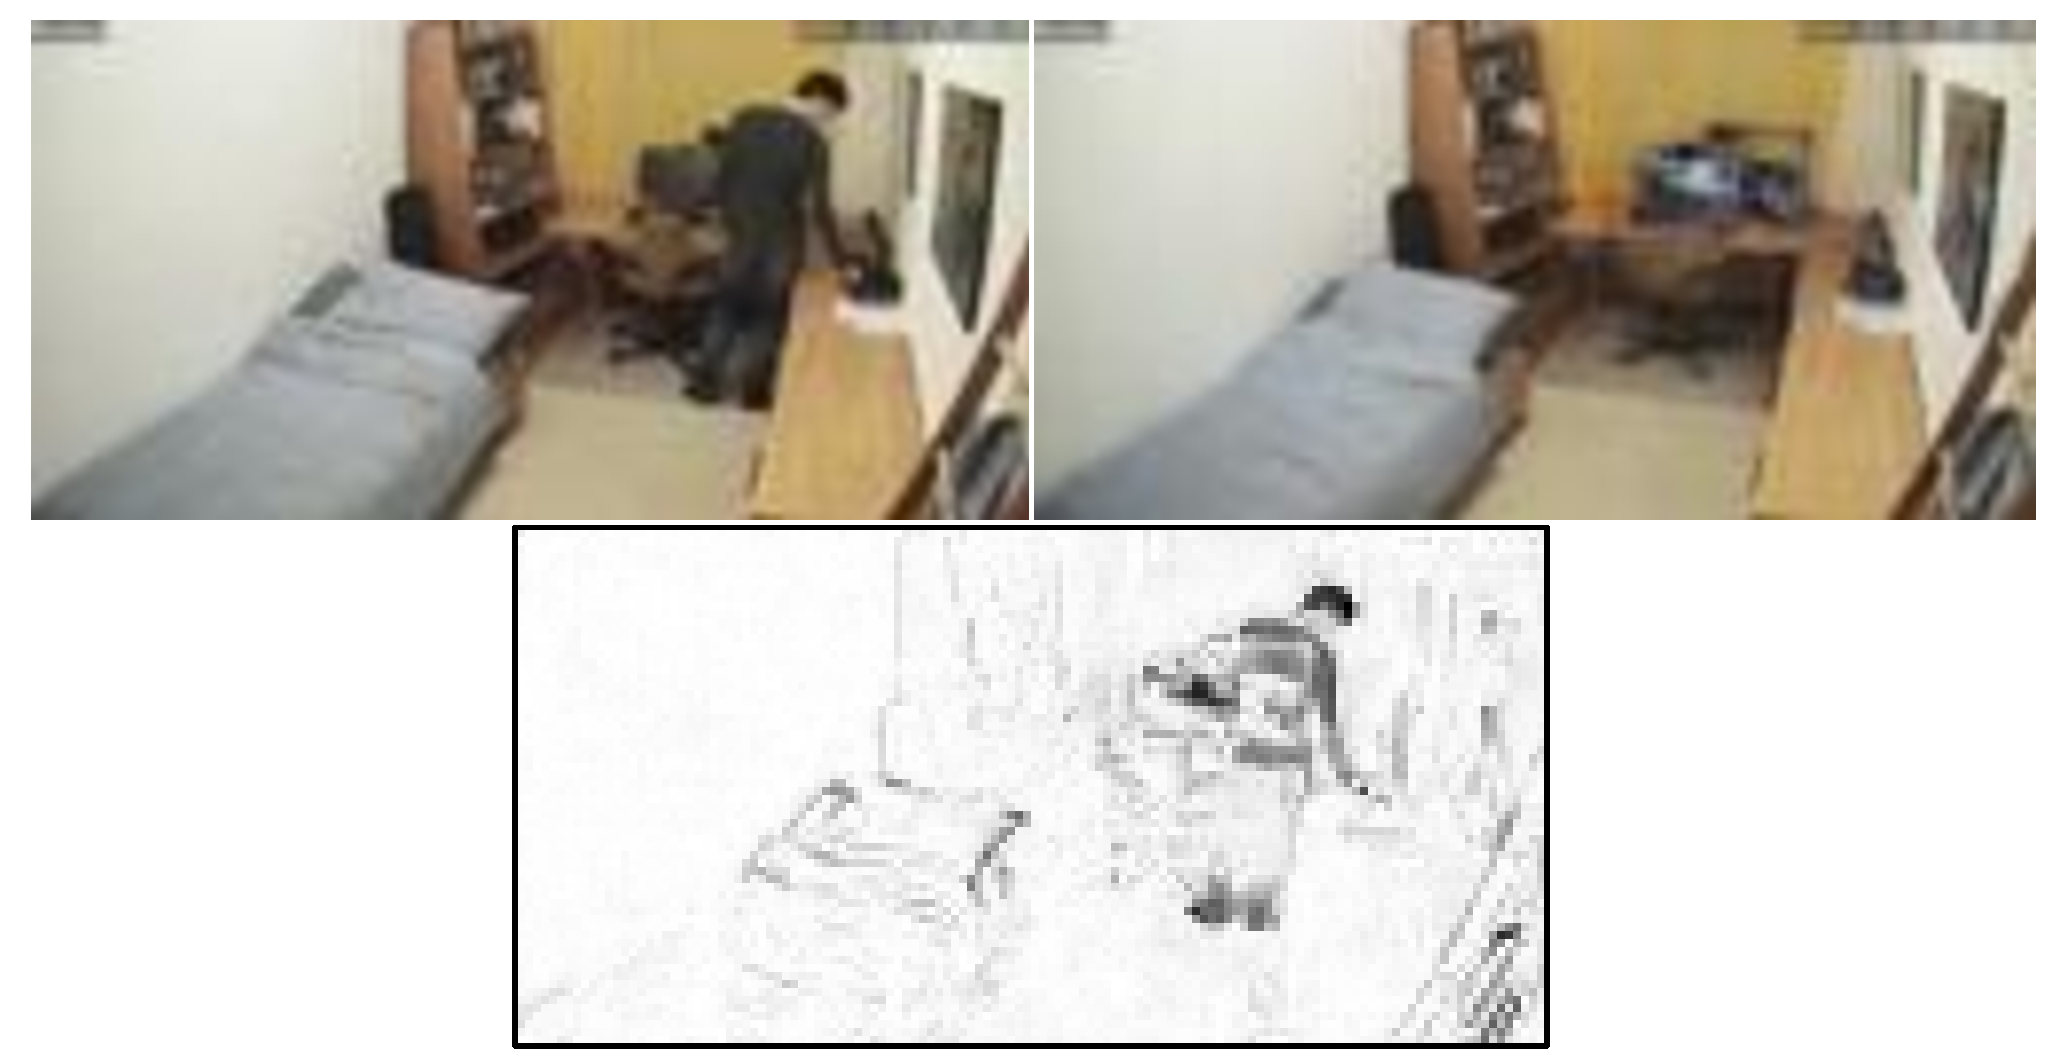
\includegraphics[width=0.8\textwidth]{graphics/eval/heatmap/heatmap.pdf}
  \caption[Exemplary heat map of the mean absolute error per pixel of a predicted frame.]{Exemplary heat map of the mean absolute error per pixel of a predicted frame. The heat map can be computed by comparing the actual frame (upper left) to the predicted future (upper right).}
  \label{fig:prediction_comparison}
\end{figure}

While the mentioned criteria can also be used to discriminate different models quickly, a qualitative evaluation of the predicted future is still missing. Evaluating a prediction is difficult as the future is uncertain and there are several if not infinite plausible outcomes that can be inferred from the past. Even for our next-frame prediction model, the 8th out of seven frames can take multiple shapes and it would be naive to simply compare the prediction to the actual observation and evaluate the model's quality based on that. On the other hand, the next-frame prediction models are integrated into IFTM and their predictions are compared to the actual frames. As explained in Section \ref{sec:vad}, the difference between the two is computed using the L1 distance and a threshold is applied to it to map the number to a binary classification result (normal, anomaly). Thus any prediction model should predict a future closely resembling the actual one or IFTM will interpret such a prediction as an indicator for an anomaly. Therefore the prediction error function $\Delta(x_{t})$ for IFTM with C-VGAN, is extended for evaluation purposes to compute the error per pixel and not over the entire frame, as shown in Equation \ref{eq:mae_pixel}. This averages the absolute prediction error of each color channel ($r$, $g$, $b$) of a single pixel, which then can be displayed as a grayscale heat map that highlights regions in a frame that the prediction model failed to model accurately. Figure \ref{fig:prediction_comparison} illustrates an example of such a heat map.

\begin{equation} \label{eq:mae_pixel}
L = \frac{| r - \hat{r} | + | g - \hat{g} | + | b - \hat{b} |}{3}
\end{equation}

Using the synthetic video outputs of the generator and their respective predicted frames' heat maps of the errors, evaluation on the models' prediction quality is done using the evaluation data set. Knowing it contains both normal and anomalous frames, we want to examine how closely the model is able to resemble the actual future (and not just any plausible outcome) and how it handles anomalous input videos. Although in other use cases, a prediction model should strive for generalization, for IFTM the next-frame prediction models must be unable to predict anomalous observations. Evaluating the predictions' quality on the evaluation data set is therefore especially helpful not only for C-VGAN but also IFTM, as they directly influence the anomaly detection results of the VAD model and the resulting metrics. Consequently there is some overlap in the presentation of the results in the following section and in the VAD results in Section \ref{subsec:vad_results}. The two results are correlated with each other and further discussed in Section \ref{sec:discussion}.


% C-VGAN Results
\subsection{Results} \label{subsec:cvgan_results} % 5 Pages

\paragraph{Training and Model Losses}
As suspected during the initial design of our modified C-VGAN architecture (see Section \ref{subsec:vgan_mod_2}), for many configurations including the initial C-VGAN setup, the discriminator is able to model the features of real videos quicker than the generator is able to learn and fake them. This is because the generator has to not only generate synthetic videos, but these videos have to reconstruct $7$ input frames with the 8th one being extrapolated from them. So the generator learns the reconstruction of past frames and the extrapolation at the same time. Meanwhile its counterpart learns to focus on the extrapolation from frame 1--7 to the 8th one, since the reconstruction of the past frames is covered by a loss term independent from the discriminator's performance. 

\begin{figure}
  \centering
  
  \begin{subfigure}{\linewidth}
    \centering
		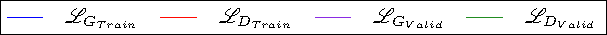
\includegraphics[width=0.6\linewidth]{{graphics/eval/cvgan_2/losses/loss_legend}.pdf}
	\end{subfigure}
	\vspace{0.01cm}
	
	\begin{subfigure}{0.32\linewidth}
	  \centering
		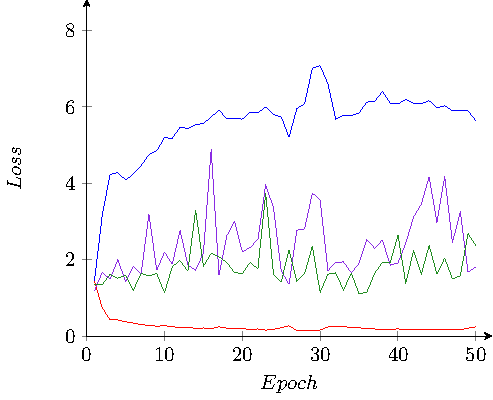
\includegraphics[width=\linewidth]{{graphics/eval/cvgan_2/losses/dfilter-32_ddropout-0.0_lambda-10_batchsize-64_learningrate-0.0002}.pdf}
		\vspace{-0.7cm}
		\caption{cf=32, dr=0.0, $\lambda$=10, bs=64, lr=2e-4}
		\label{subfig:cf=32-dr=0.0-l=10-bs=64-lr=2e-4-loss-1}
	\end{subfigure}
	\hfill
	\begin{subfigure}{0.32\linewidth}
	  \centering
		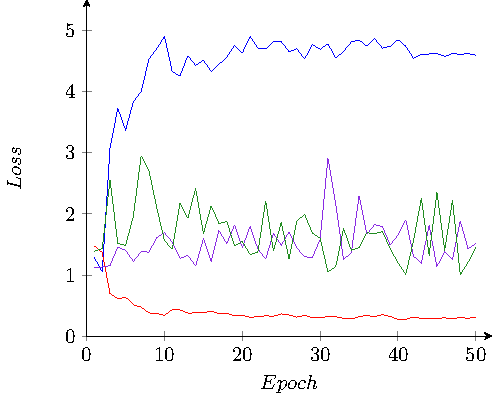
\includegraphics[width=\linewidth]{{graphics/eval/cvgan_2/losses/dfilter-16_ddropout-0.0_lambda-10_batchsize-64_learningrate-0.0002}.pdf}
		\vspace{-0.7cm}
		\caption{cf=16, dr=0.0, $\lambda$=10, bs=64, lr=2e-4}
		\label{subfig:cf=16-dr=0.0-l=10-bs=64-lr=2e-4-loss-1}
	\end{subfigure}
  \hfill
  \begin{subfigure}{0.32\linewidth}
    \centering
		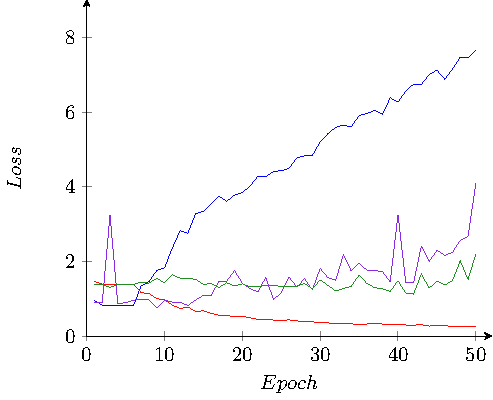
\includegraphics[width=\linewidth]{{graphics/eval/cvgan_2/losses/dfilter-16_ddropout-0.3_lambda-5_batchsize-64_learningrate-0.0002}.pdf}
		\vspace{-0.7cm}
		\caption{cf=16, dr=0.3, $\lambda$=5, bs=64, lr=2e-4}
		\label{subfig:cf=16-dr=0.3-l=5-bs=64-lr=2e-4-loss-1}
	\end{subfigure}
	
	\begin{subfigure}{0.32\linewidth}
	  \centering
		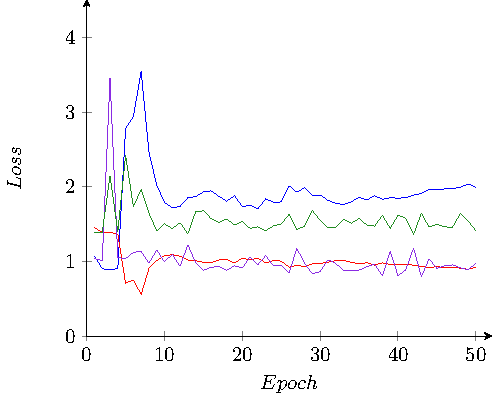
\includegraphics[width=\linewidth]{{graphics/eval/cvgan_2/losses/dfilter-16_ddropout-0.3_lambda-8_batchsize-64_learningrate-0.0002}.pdf}
		\vspace{-0.7cm}
		\caption{cf=16, dr=0.3, $\lambda$=8, bs=64, lr=2e-4}
		\label{subfig:cf=16-dr=0.3-l=8-bs=64-lr=2e-4-loss-1}
	\end{subfigure}
  \hfill
  \begin{subfigure}{0.32\linewidth}
	  \centering
		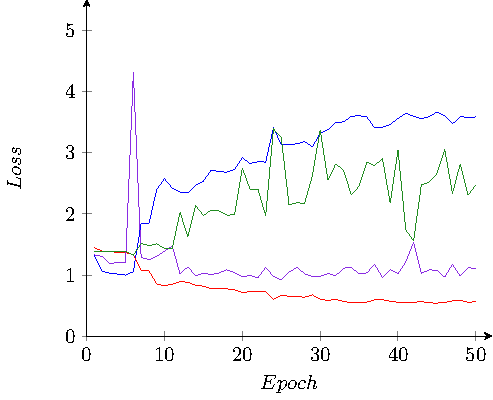
\includegraphics[width=\linewidth]{{graphics/eval/cvgan_2/losses/dfilter-16_ddropout-0.3_lambda-14_batchsize-64_learningrate-0.0002}.pdf}
		\vspace{-0.7cm}
		\caption{cf=16, dr=0.3, $\lambda$=14, bs=64, lr=2e-4}
		\label{subfig:cf=16-dr=0.3-l=14-bs=64-lr=2e-4-loss-1}
	\end{subfigure}
	\hfill
	\begin{subfigure}{0.32\linewidth}
	  \centering
		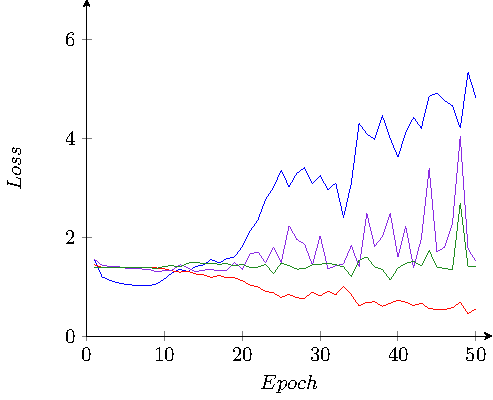
\includegraphics[width=\linewidth]{{graphics/eval/cvgan_2/losses/dfilter-16_ddropout-0.3_lambda-20_batchsize-64_learningrate-0.0002}.pdf}
		\vspace{-0.7cm}
		\caption{cf=16, dr=0.3, $\lambda$=20, bs=64, lr=2e-4}
		\label{subfig:cf=16-dr=0.3-l=20-bs=64-lr=2e-4-loss-1}
	\end{subfigure}  
		
	\caption[C-VGANs' training and validation losses over the epochs. (1)]{Training and validation losses ($\mathcal{L}$) over the epochs of generator ($G$) and discriminator ($D$) of C-VGAN for next-frame prediction using different hyperparameters. Note that higher losses do not necessarily imply a decrease in model quality; generator and discriminator should reach an equilibrium in their respective losses, with both of the models improving in parallel.}
	\label{fig:cvgan_losses_1}
\end{figure}

As a result, for the default configuration of the discriminator and with no dropout for each of its layers' outputs, not a single stable configuration was found. In every scenario, the discriminator overpowers the generator in the first 5--10 epochs, its loss converging towards $0$. Consequently the total generator loss quickly increases until its first loss term converges to its maximum value --- it is the negated second term of the discriminator loss term. The reconstruction loss term also falls into a local optimum and does not recover. This is to be expected as it is a known failure mode, in which the generator no longer improves in any way or actively degrades in quality (see Section \ref{sec:gans}). However this failure mode, as explained in the methodology in the previous section, can be quickly detected and training of such a C-VGAN configuration can be stopped early on, with the models being discarded. However for completeness sake, the default configuration was run for all $50$ epochs and its losses are depicted in Figure \ref{subfig:cf=32-dr=0.0-l=10-bs=64-lr=2e-4-loss-1}. It is to note, that in this configuration, while generator and discriminator training losses are both converging respectively, their validation losses behave differently: The discriminator loss on the validation dataset on every epoch is much higher and is fluctuating. This is an indicator for an overfitting discriminator model. This is further supported by the lower generator validation loss, as the discriminator can not distinguish synthetic and real videos extrapolated and drawn from the validation split, as it overfits the training split.

Consequently, attempts were made to impair the discriminator so the generator will manage to keep up with it. This was first done by reducing its convolutional filters on every layer ($cf$ parameter, see Section \ref{subsec:framework_cvgan}), so the discriminator is less able to contain every feature representation of real and synthetic videos. The result can be seen in Figure \ref{subfig:cf=16-dr=0.0-l=10-bs=64-lr=2e-4-loss-1}, with an overall smaller validation loss for both models. But the discriminator still overpowers the generator to some degree and overfits the training split, having a much higher validation loss than training loss. Configurations using the same parameters for the discriminator also behave that way, hence their training was stopped after epoch 10--20 when it became apparent. Next a dropout rate to the discriminator's layers was introduced ($dr$ parameter). And, in combination to the impairment in its convolutional filters, a stable equilibrium was found: Shown in Figure \ref{subfig:cf=16-dr=0.3-l=10-bs=64-lr=2e-4-loss-2}, after an initial spike in the generator loss accompanied by a drop in the discriminator's, the losses reach an equilibrium after epoch $20$. The validation split losses are also more stable, atleast for the discriminator. The generator validation loss has still an upward trend and when inspecting the generator training loss values closely, we noticed a small increase over the last epochs as well. Note this is not unusual, as the convergence for GANs is often not a stable state. The discriminator's feedback get less meaningful over time, causing the generator to optimize its parameters based on random feedback. 

\begin{figure}
  \centering
  
  \begin{subfigure}{\linewidth}
    \centering
		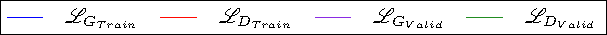
\includegraphics[width=0.6\linewidth]{{graphics/eval/cvgan_2/losses/loss_legend}.pdf}
	\end{subfigure}
	\vspace{0.01cm}
	
	\begin{subfigure}{0.32\linewidth}
	  \centering
		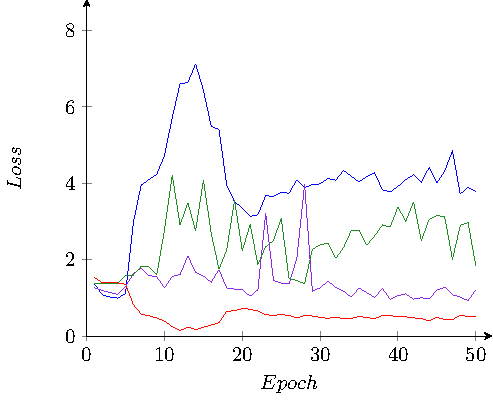
\includegraphics[width=\linewidth]{{graphics/eval/cvgan_2/losses/dfilter-16_ddropout-0.3_lambda-10_batchsize-256_learningrate-0.0004}.pdf}
		\vspace{-0.7cm}
		\caption{cf=16, dr=0.3, $\lambda$=10, bs=256, lr=4e-4}
		\label{subfig:cf=16-dr=0.3-l=10-bs=256-lr=4e-4-loss-2}
	\end{subfigure}
	\hfill
	\begin{subfigure}{0.32\linewidth}
	  \centering
		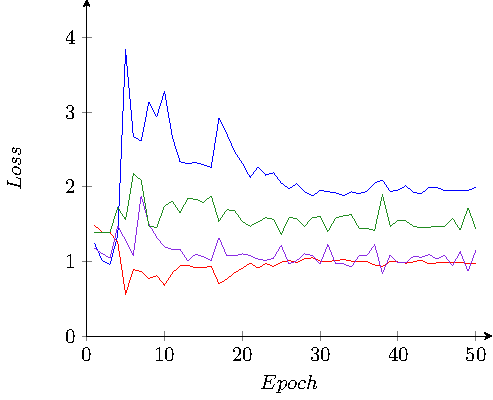
\includegraphics[width=\linewidth]{{graphics/eval/cvgan_2/losses/dfilter-16_ddropout-0.3_lambda-10_batchsize-128_learningrate-0.00028}.pdf}
		\vspace{-0.7cm}
		\caption{cf=16, dr=0.3, $\lambda$=10, bs=128, lr=2.8e-4}
		\label{subfig:cf=16-dr=0.3-l=10-bs=128-lr=2.8e-4-loss-2}
	\end{subfigure}
	\hfill
	\begin{subfigure}{0.32\linewidth}
	  \centering
		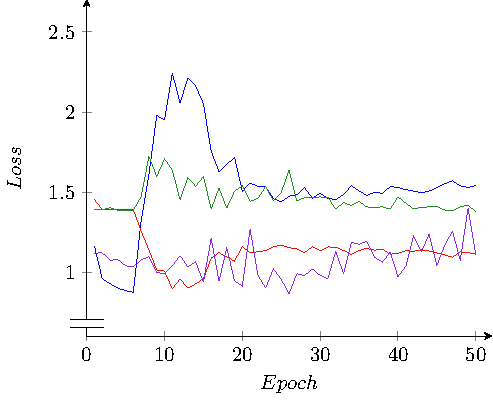
\includegraphics[width=\linewidth]{{graphics/eval/cvgan_2/losses/dfilter-16_ddropout-0.3_lambda-10_batchsize-64_learningrate-0.0002}.pdf}
		\vspace{-0.7cm}
		\caption{cf=16, dr=0.3, $\lambda$=10, bs=64, lr=2e-4}
		\label{subfig:cf=16-dr=0.3-l=10-bs=64-lr=2e-4-loss-2}
	\end{subfigure}
	
	\begin{subfigure}{0.32\linewidth}
	  \centering
		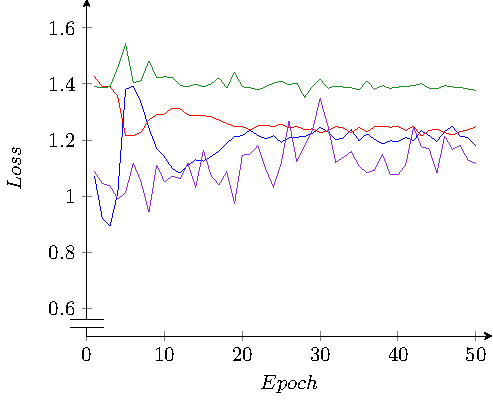
\includegraphics[width=\linewidth]{{graphics/eval/cvgan_2/losses/dfilter-16_ddropout-0.3_lambda-10_batchsize-32_learningrate-0.0002}.pdf}
		\vspace{-0.7cm}
		\caption{cf=16, dr=0.3, $\lambda$=10, bs=32, lr=2e-4}
		\label{subfig:cf=16-dr=0.3-l=10-bs=32-lr=2e-4-loss-2}
	\end{subfigure}
	\hfill
	\begin{subfigure}{0.32\linewidth}
	  \centering
		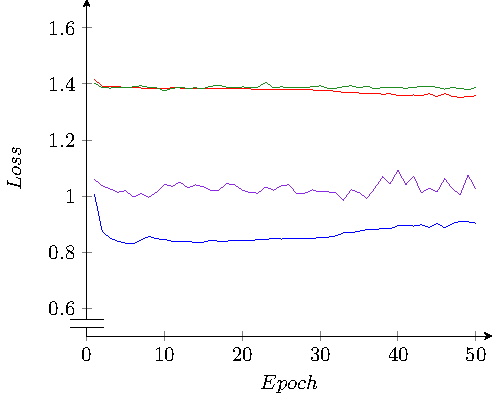
\includegraphics[width=\linewidth]{{graphics/eval/cvgan_2/losses/dfilter-16_ddropout-0.3_lambda-10_batchsize-16_learningrate-0.0002}.pdf}
		\vspace{-0.7cm}
		\caption{cf=16, dr=0.3, $\lambda$=10, bs=16, lr=2e-4}
		\label{subfig:cf=16-dr=0.3-l=10-bs=16-lr=2e-4-loss-2}
	\end{subfigure}
	\hfill
	\begin{subfigure}{0.32\linewidth}
	  \centering
		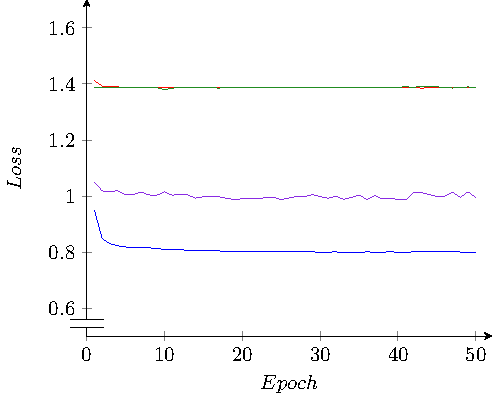
\includegraphics[width=\linewidth]{{graphics/eval/cvgan_2/losses/dfilter-16_ddropout-0.3_lambda-10_batchsize-8_learningrate-0.0002}.pdf}
		\vspace{-0.7cm}
		\caption{cf=16, dr=0.3, $\lambda$=10, bs=8, lr=2e-4}
		\label{subfig:cf=16-dr=0.3-l=10-bs=8-lr=2e-4-loss-2}
	\end{subfigure}
			
	\caption[C-VGANs' training and validation losses over the epochs. (2)]{Training and validation losses ($\mathcal{L}$) over the epochs of generator ($G$) and discriminator ($D$) of C-VGAN for next-frame prediction using different hyperparameters. Note that higher losses do not necessarily imply a decrease in model quality; generator and discriminator should reach an equilibrium in their respective losses, with both of the models improving in parallel.}
	\label{fig:cvgan_losses_2}
\end{figure}

\begin{figure}
  \centering

	\begin{subfigure}{\textwidth}
		\centering
		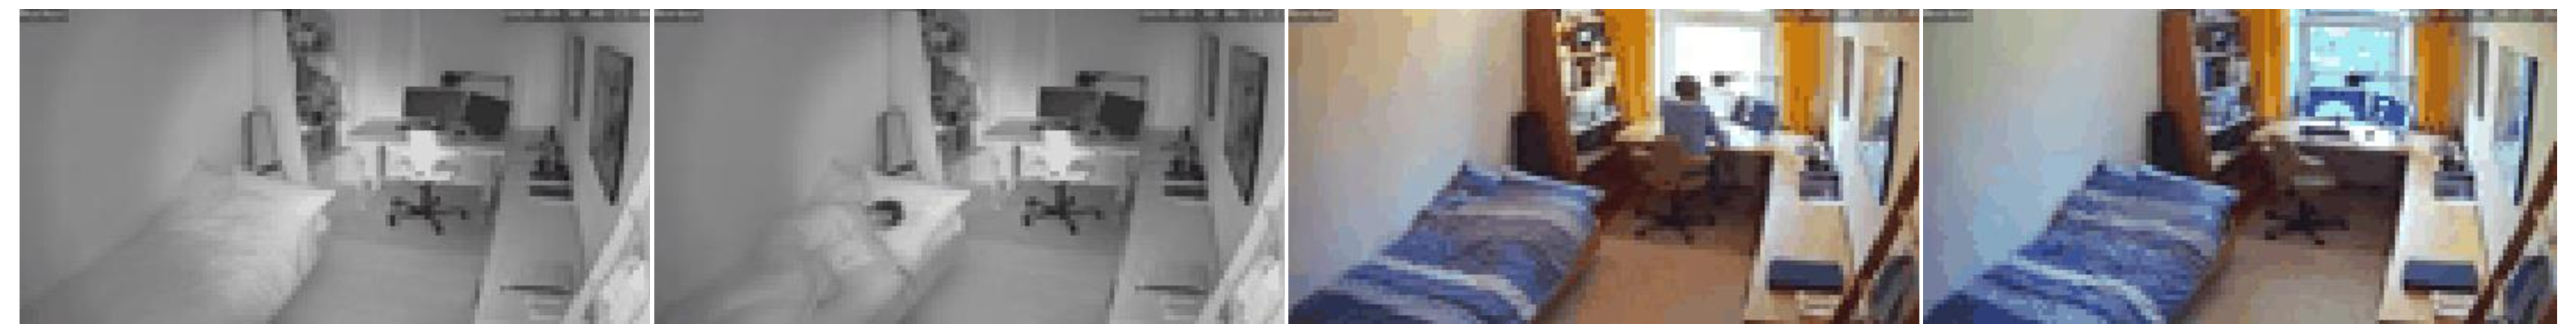
\includegraphics[width=\textwidth]{graphics/eval/cvgan_2/qual_basic/actual/actual.pdf}
	  \caption{Actual next frames.}
	  \label{subfig:cvgan_comparison_lambda}
	\end{subfigure}

	\begin{subfigure}{\textwidth}
		\centering
		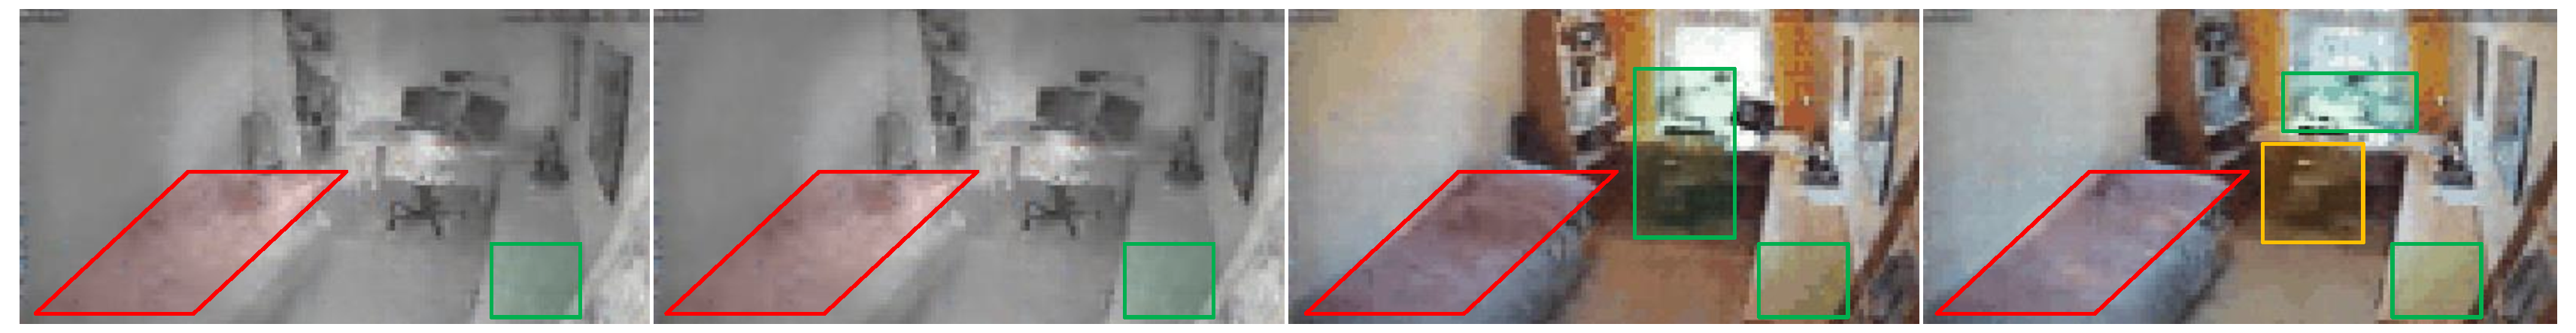
\includegraphics[width=\textwidth]{graphics/eval/cvgan_2/qual_basic/dfilter-16_ddropout-0.3_lambda-5_batchsize-64_learningrate-0.0002/predicted.pdf}
	  \caption{cf=16, dr=0.3, $\lambda$=5, bs=64, lr=2e-4}
	  \label{subfig:l5-comp-1}
	\end{subfigure}

	\begin{subfigure}{\textwidth}
		\centering
		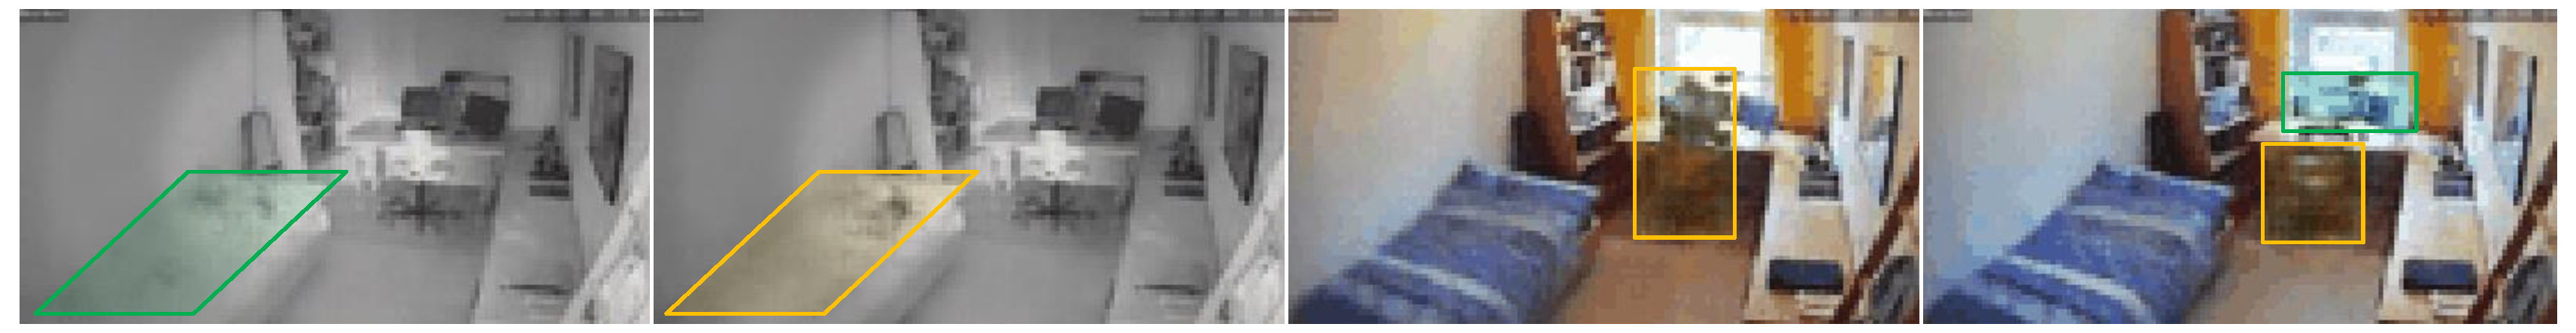
\includegraphics[width=\textwidth]{graphics/eval/cvgan_2/qual_basic/dfilter-16_ddropout-0.3_lambda-8_batchsize-64_learningrate-0.0002/predicted.pdf}
	  \caption{cf=16, dr=0.3, $\lambda$=8, bs=64, lr=2e-4}
	  \label{subfig:l8-comp-1}
	\end{subfigure}

	\begin{subfigure}{\textwidth}
		\centering
		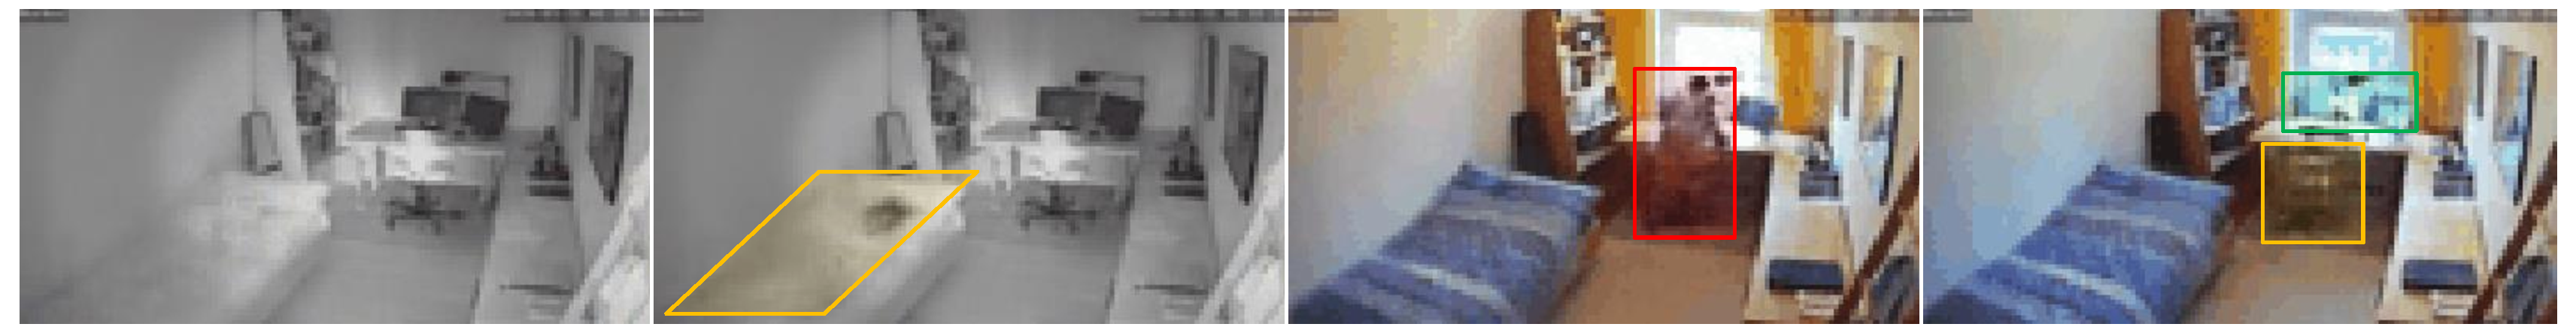
\includegraphics[width=\textwidth]{graphics/eval/cvgan_2/qual_basic/dfilter-16_ddropout-0.3_lambda-10_batchsize-64_learningrate-0.0002/predicted.pdf}
	  \caption{cf=16, dr=0.3, $\lambda$=10, bs=64, lr=2e-4}
	  \label{subfig:l10-comp-1}
	\end{subfigure}

	\begin{subfigure}{\textwidth}
		\centering
		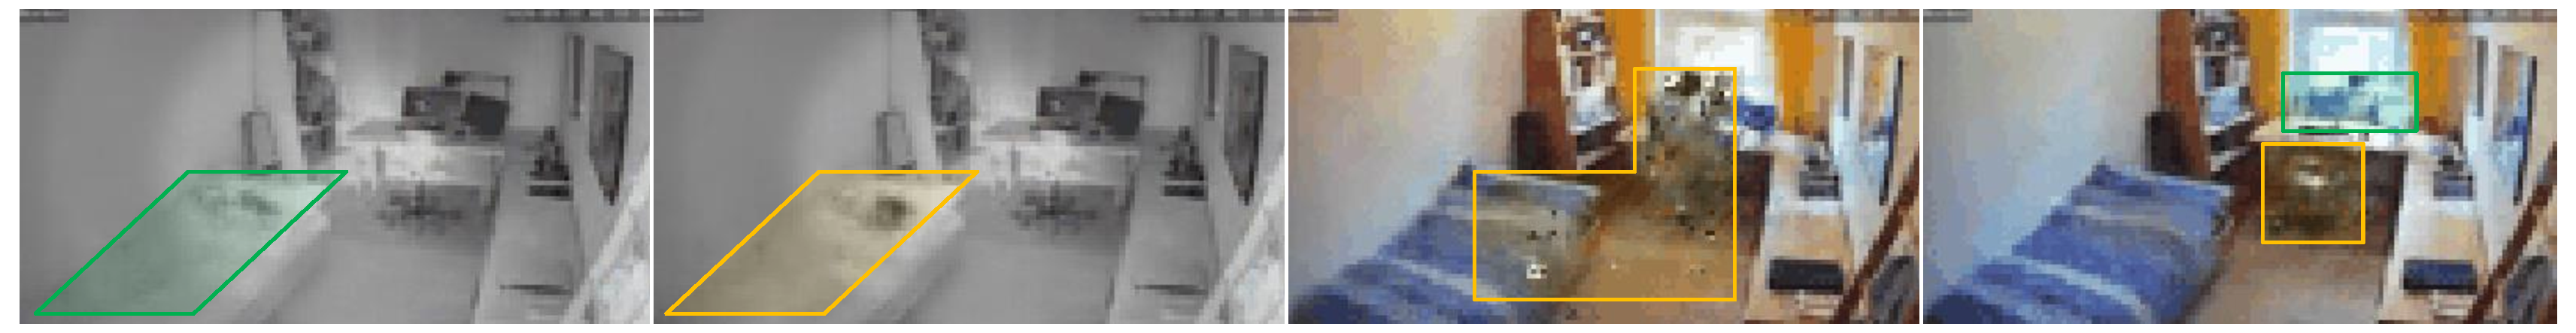
\includegraphics[width=\textwidth]{graphics/eval/cvgan_2/qual_basic/dfilter-16_ddropout-0.3_lambda-14_batchsize-64_learningrate-0.0002/predicted.pdf}
	  \caption{cf=16, dr=0.3, $\lambda$=14, bs=64, lr=2e-4}
	  \label{subfig:l14-comp-1}
	\end{subfigure}
	
	\caption[Qualitative comparison between different C-VGAN models. (1)]{Comparison between the actual next frames of video clips (a) and their respective predictions by C-VGAN models that were trained using different weights ($\lambda$) for their reconstruction loss term. Marked in red one can see how different object patterns are collapsed into the same pattern. Omitted or hallucinated objects are colored in green, and objects that lack detail or are not fully constructed are marked yellow.}
	\label{fig:cvgan_comparison_lambda}
\end{figure}

Following the discovery of a configuration that accomplishes an equilibrium, attempts were made to fine tune the parameter $\lambda$, regulating how much the input frames determine the output, but this either ruined the balance of the two models --- see Figure \ref{fig:cvgan_losses_1} for some of the attempt's results, or worsened the quality of the output. The latter will be further assessed during the presentation of the qualitative evaluation. Tuning the batch size however produced mixed results, depicted in Figure \ref{fig:cvgan_losses_2}: Increasing it and with it the learning rate, on one hand sped up training, but on the other resulted in generally higher overall losses. Although this is not necessarily bad as long as models improve in parallel, it requires further qualitative evaluation of the model's outputs. Meanwhile, when greatly decreasing the batch size but keeping the learning rate fixed, convergence of the losses is not only faster but extremely stable. This is not only for the case for the training losses but also for the validation split. In case of the discriminator, validation and training loss are practically identical when using a batch size of $16$ and $8$, with a slight upward and downward trend for the generator and discriminator training losses after epoch $30$, respectively, for a batch size of $16$. See Figure \ref{subfig:cf=16-dr=0.3-l=10-bs=16-lr=2e-4-loss-2} and \ref{subfig:cf=16-dr=0.3-l=10-bs=8-lr=2e-4-loss-2}. This is a sign for great generalization. For the generator, validation loss is still higher, which means it is not able to reconstruct unknown frames as well as ones that were witnessed during training. Even so, both generator losses are still lower with smaller training batches than when using any other configuration. This confirms our hypothesis from Section \ref{subsec:framework_cvgan}, that while higher batch sizes are a good tool to help with generalization and drown out sparse anomalies in the training data set, they are also hurting the model to learn less frequently occurring object patterns. In addition, smaller batches also seem to help the generator to keep up with its counterpart: Giving the discriminator less examples per step is an indirect impairment to its training process, because the model is smaller and can more quickly adapt to the observations witnessed in a step. Limiting that is especially crucial in the initial epochs, because this is when the generator loss peaks in other configurations before converging to a lower value. Preventing this early overpowering, that might put the generator into a bad local minimum, also improves the generator's overall quality.

Finally for the configurations that are still in a balance after $50$ epochs there could be better results if one were to train those further. Nonetheless for the scope of this evaluation and due to the high time cost, training was stopped at that point with the option to evaluate the other models from their earlier epochs before their respective loss equilibria were lost and they had regressed in quality.

\paragraph{Qualitative Results}

\begin{figure}
  \centering

	\begin{subfigure}{\textwidth}
		\centering
		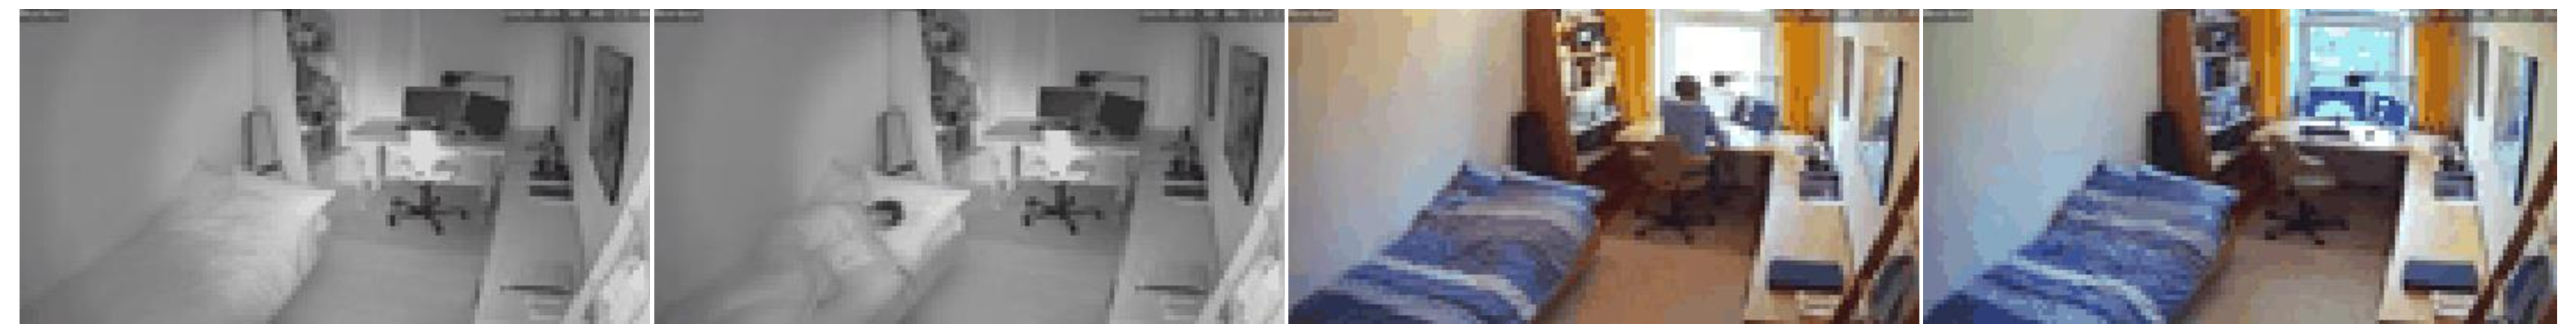
\includegraphics[width=\textwidth]{graphics/eval/cvgan_2/qual_basic/actual/actual.pdf}
	  \caption{Actual next frames.}
	  \label{subfig:cvgan_comparison_bs}
	\end{subfigure}
	
	\begin{subfigure}{\textwidth}
	  \centering
		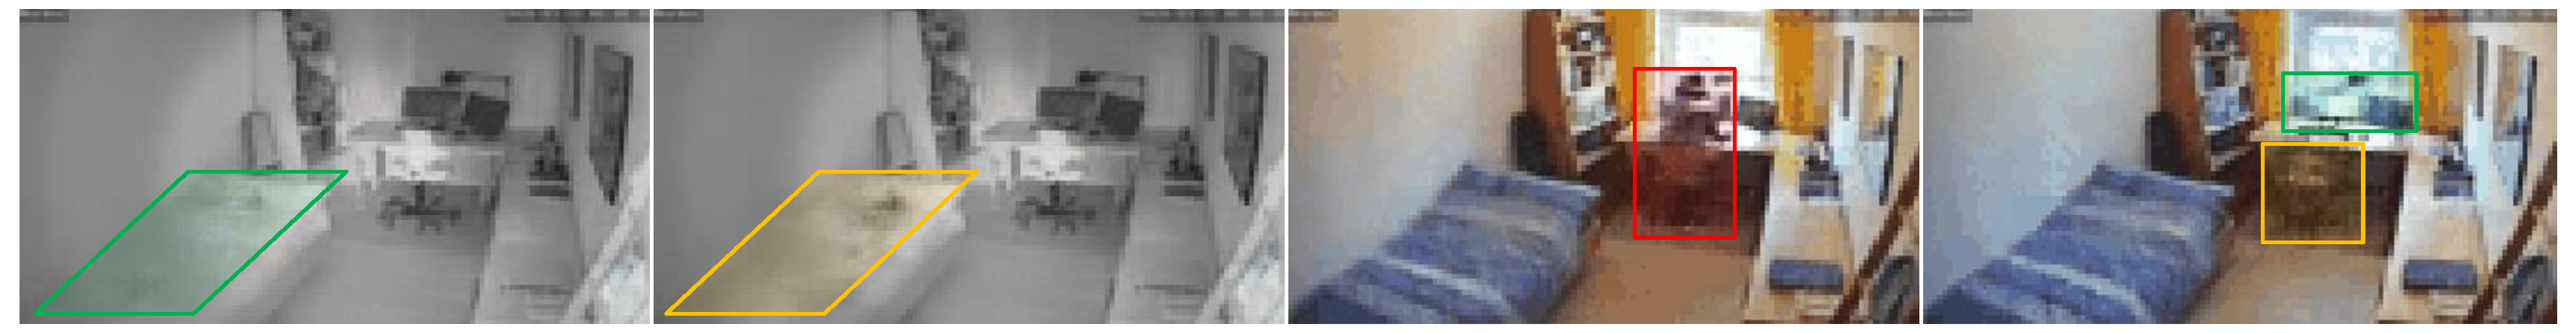
\includegraphics[width=\textwidth]{graphics/eval/cvgan_2/qual_basic/dfilter-16_ddropout-0.3_lambda-10_batchsize-128_learningrate-0.00028/predicted.pdf}
		\caption{cf=16, dr=0.3, $\lambda$=10, bs=128, lr=2.8e-4}
		\label{subfig:bs128-comp-2}
	\end{subfigure}

	\begin{subfigure}{\textwidth}
		\centering
		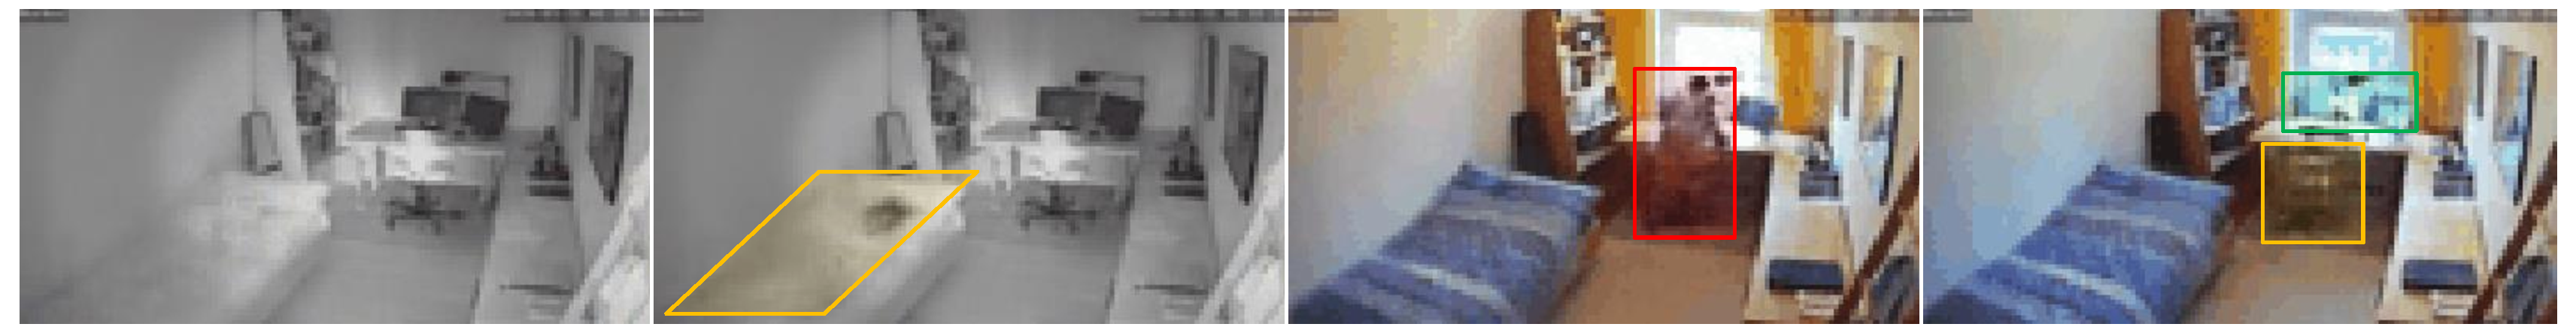
\includegraphics[width=\textwidth]{graphics/eval/cvgan_2/qual_basic/dfilter-16_ddropout-0.3_lambda-10_batchsize-64_learningrate-0.0002/predicted.pdf}
	  \caption{cf=16, dr=0.3, $\lambda$=10, bs=64, lr=2e-4}
	  \label{subfig:bs64-comp-2}
	\end{subfigure}

	\begin{subfigure}{\textwidth}
		\centering
		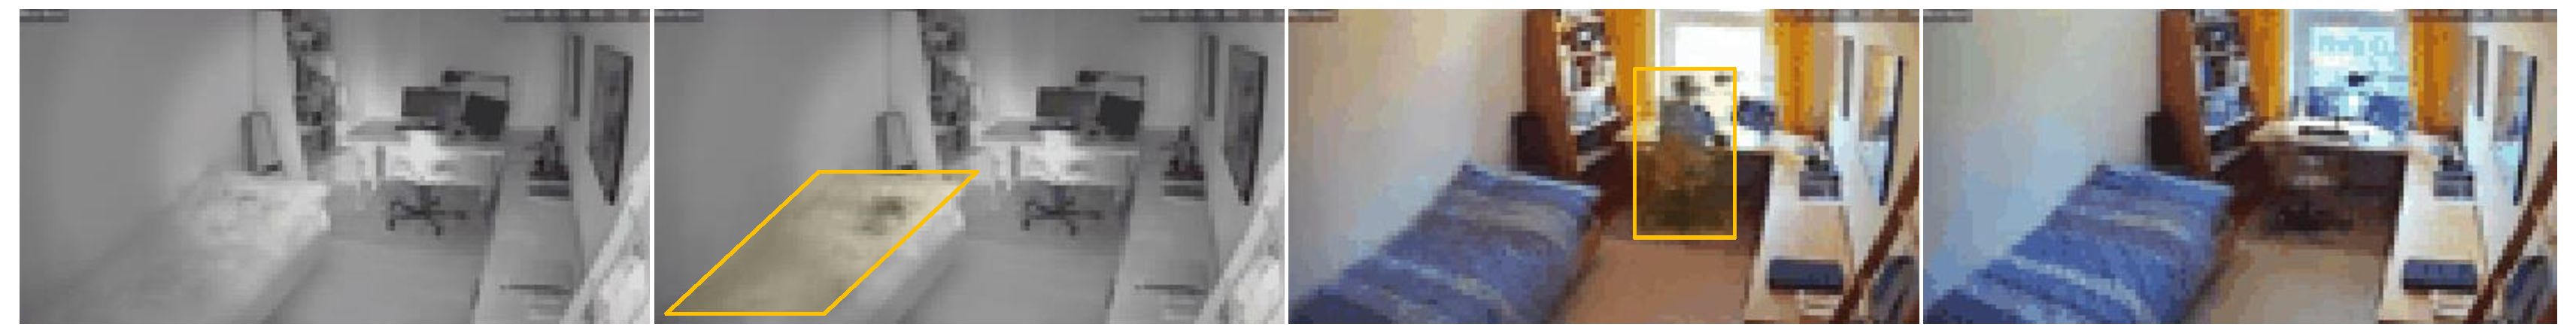
\includegraphics[width=\textwidth]{graphics/eval/cvgan_2/qual_basic/dfilter-16_ddropout-0.3_lambda-10_batchsize-32_learningrate-0.0002/predicted.pdf}
	  \caption{cf=16, dr=0.3, $\lambda$=10, bs=32, lr=2e-4}
	  \label{subfig:bs32-comp-2}
	\end{subfigure}

	\begin{subfigure}{\textwidth}
		\centering
		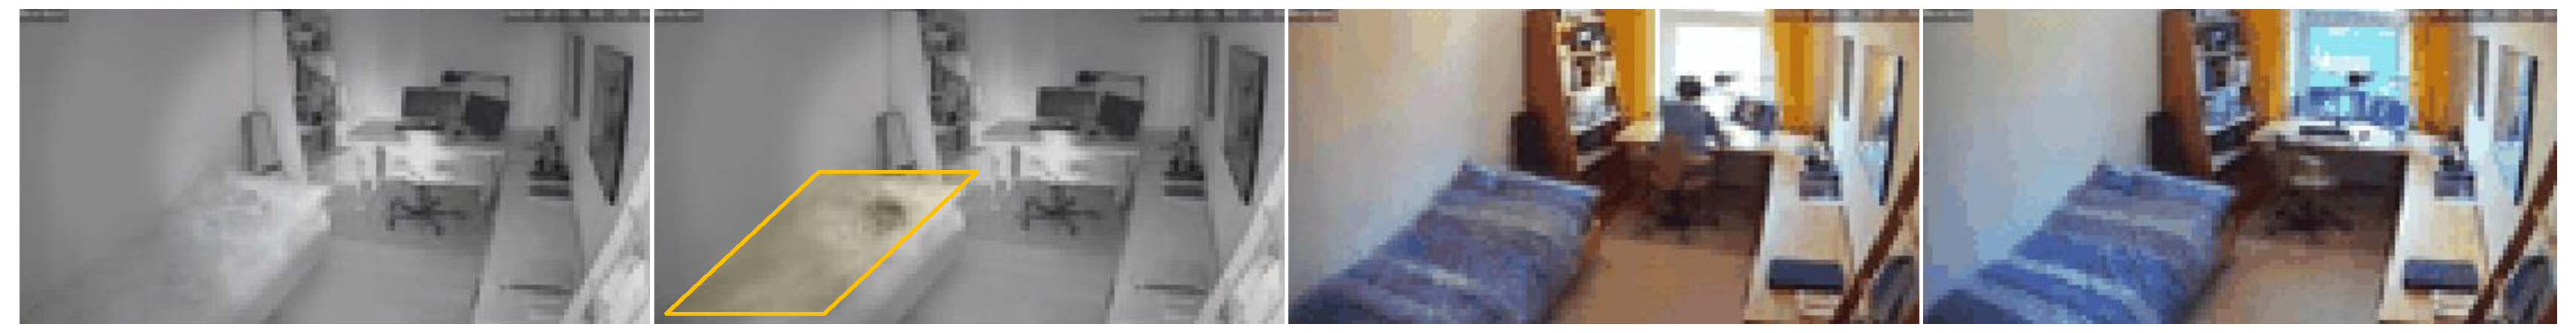
\includegraphics[width=\textwidth]{graphics/eval/cvgan_2/qual_basic/dfilter-16_ddropout-0.3_lambda-10_batchsize-16_learningrate-0.0002/predicted.pdf}
	  \caption{cf=16, dr=0.3, $\lambda$=10, bs=16, lr=2e-4}
	  \label{subfig:bs16-comp-2}
	\end{subfigure}
	
	\caption[Qualitative comparison between different C-VGAN models. (2)]{Comparison between the actual next frames of video clips (a) and their respective predictions by C-VGAN models that were trained using different batch sizes ($bs$). Marked in red one can see how different object patterns are collapsed into the same pattern. Omitted or hallucinated objects are colored in green, and objects that lack detail or are not fully constructed are marked yellow.}
	\label{fig:cvgan_comparison_bs}
\end{figure}

Since none of the configurations in which the discriminator was not impaired proved to be stable, they are not included in the qualitative assessment. Overall, their reconstructed and predicted frames were of poor quality and contained a lot of noise. They are not alone in this, as any changes to the reconstruction loss term weight ($\lambda$) also worsened the quality of the output video clips. Shown in Figure \ref{fig:cvgan_comparison_lambda}, one can see some of these configurations making next-frame predictions on the test split of the training data set. For low values of $\lambda$, hallucinations and omissions of object patterns are common, same as the collapsing of different input videos into the same outputs. Although this could still be used for IFTM if normal instances are collapsed into the same outputs while anomalous ones are not, this does not meet the requirement for a next-frame forecasting model. In contrast, giving the reconstruction loss too much weight compared to the prediction of the 8th frame, worsens its quality drastically. Depicted in Figure \ref{subfig:l14-comp-1}, the model even hallucinates a person lying in the bed when using a higher reconstruction loss weight and inserts gray noise into videos during the day. One can assume that features from observations from the night bleed into that output, causing that noise. This gets worse as the number of epochs increase, which matches the results for the model loss progression from the previous section. For the default reconstruction loss term weight ($\lambda$=10), there are fewer errors in the object patterns, with the exception of the substitution of the person's clothing and the change in posture (marked in red in Figure \ref{subfig:l10-comp-1}). This is also hint of some form of output collapse, and makes such a prediction model insufficient. Finally in all of these configurations, the computer displays on the desk often merge with the window during the day, having no clear boundary between them and the light that emits from the outside. 

The last issues disappear, along hallucination issues for the test split, once the batch size is decreased, as shown in Figure \ref{fig:cvgan_comparison_bs}: Starting with a batch size of $32$, the clothing of the person gets successfully reconstructed along with their posture, and beyond a batch size of $16$, the object pattern of the person is also indistinguishable from the one in the actual frame. The light from the window is also more true to the ground truth. Yet some inaccuracies and noise remain; for example no matter the configuration the person lying in bed is always blurry. The same is the case for the dynamic content of the computer displays on the desk, although from our point of view the latter difference is negligible (see Figure \ref{subfig:bs16-comp-2}).

\begin{figure}
  \centering

	\begin{subfigure}{\textwidth}
		\centering
		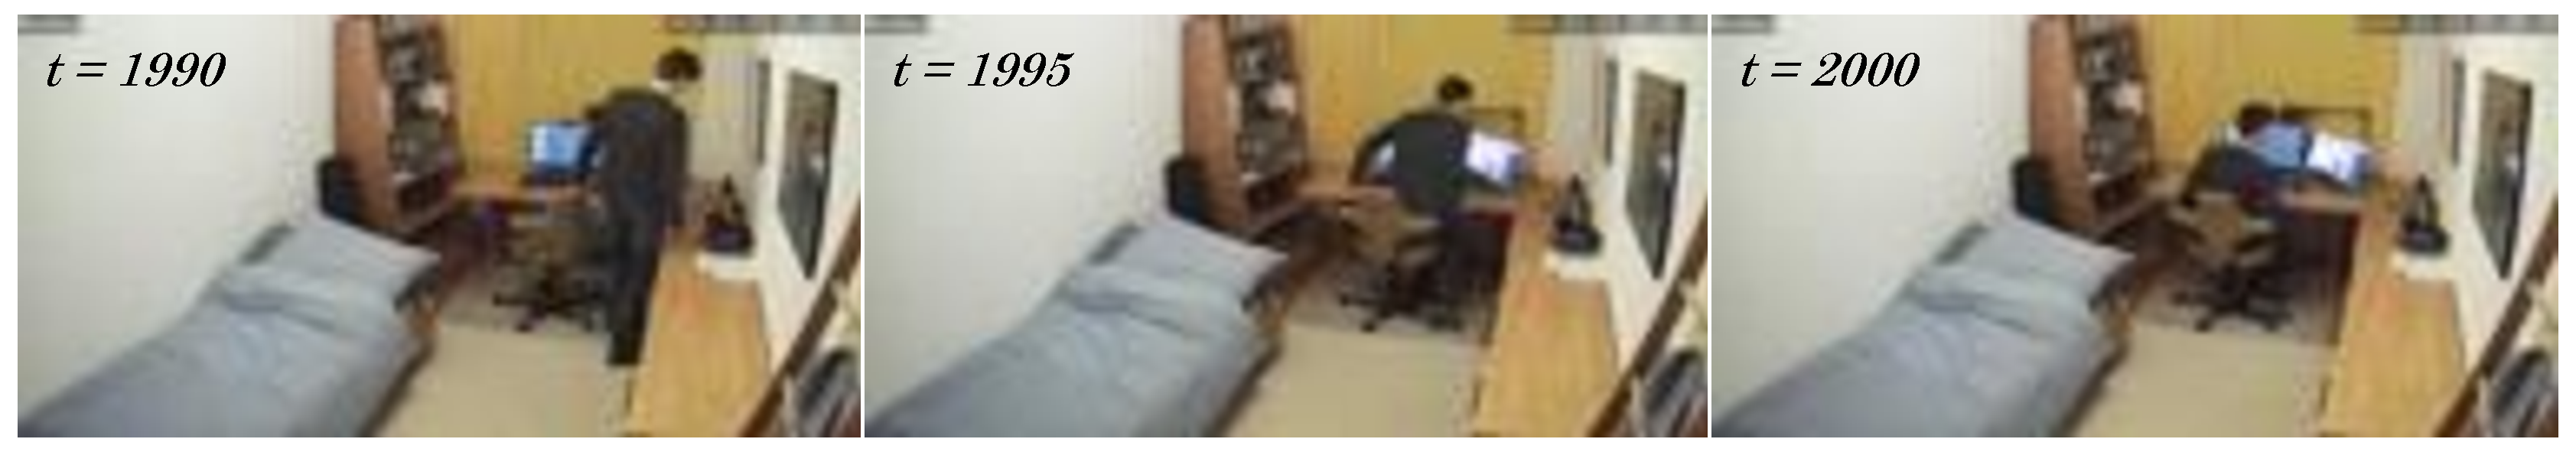
\includegraphics[width=0.9\textwidth]{graphics/eval/cvgan_2/qual_prediction/real/normal.pdf}
	  \caption{Actual next frames.}
	  \label{subfig:cvgan_prediction_normal}
	\end{subfigure}
	
	\begin{subfigure}{\textwidth}
	  \centering
		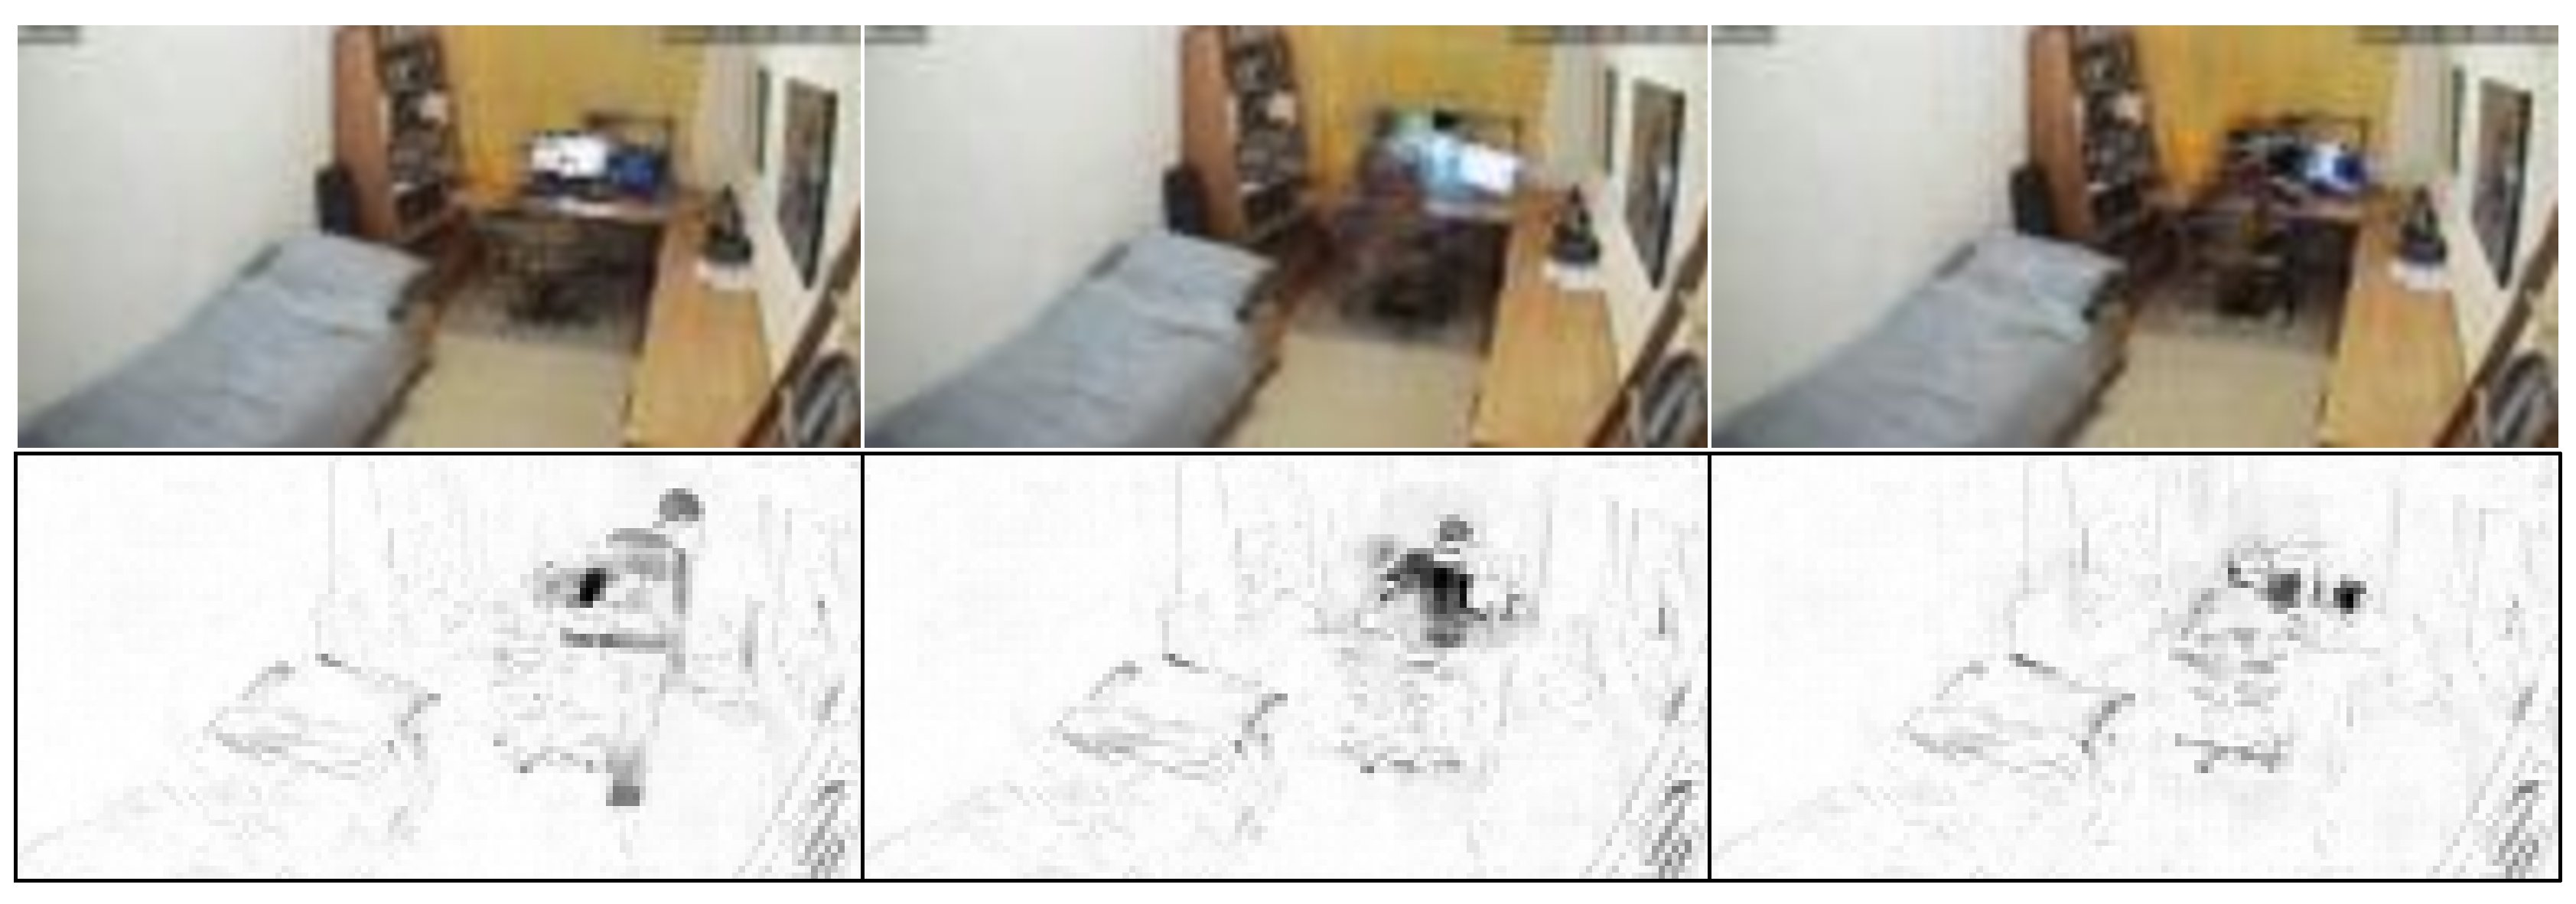
\includegraphics[width=0.9\textwidth]{graphics/eval/cvgan_2/qual_prediction/cvgan_2_dfilter-16_ddropout-0.3_lambda-10_batchsize-128_learningrate-0.000282842712474619_epochs-0050/normal.pdf}
		\caption{cf=16, dr=0.3, $\lambda$=10, bs=128, lr=2.8e-4}
		\label{subfig:bs128-pred-n}
	\end{subfigure}	
	
	\begin{subfigure}{\textwidth}
	  \centering
		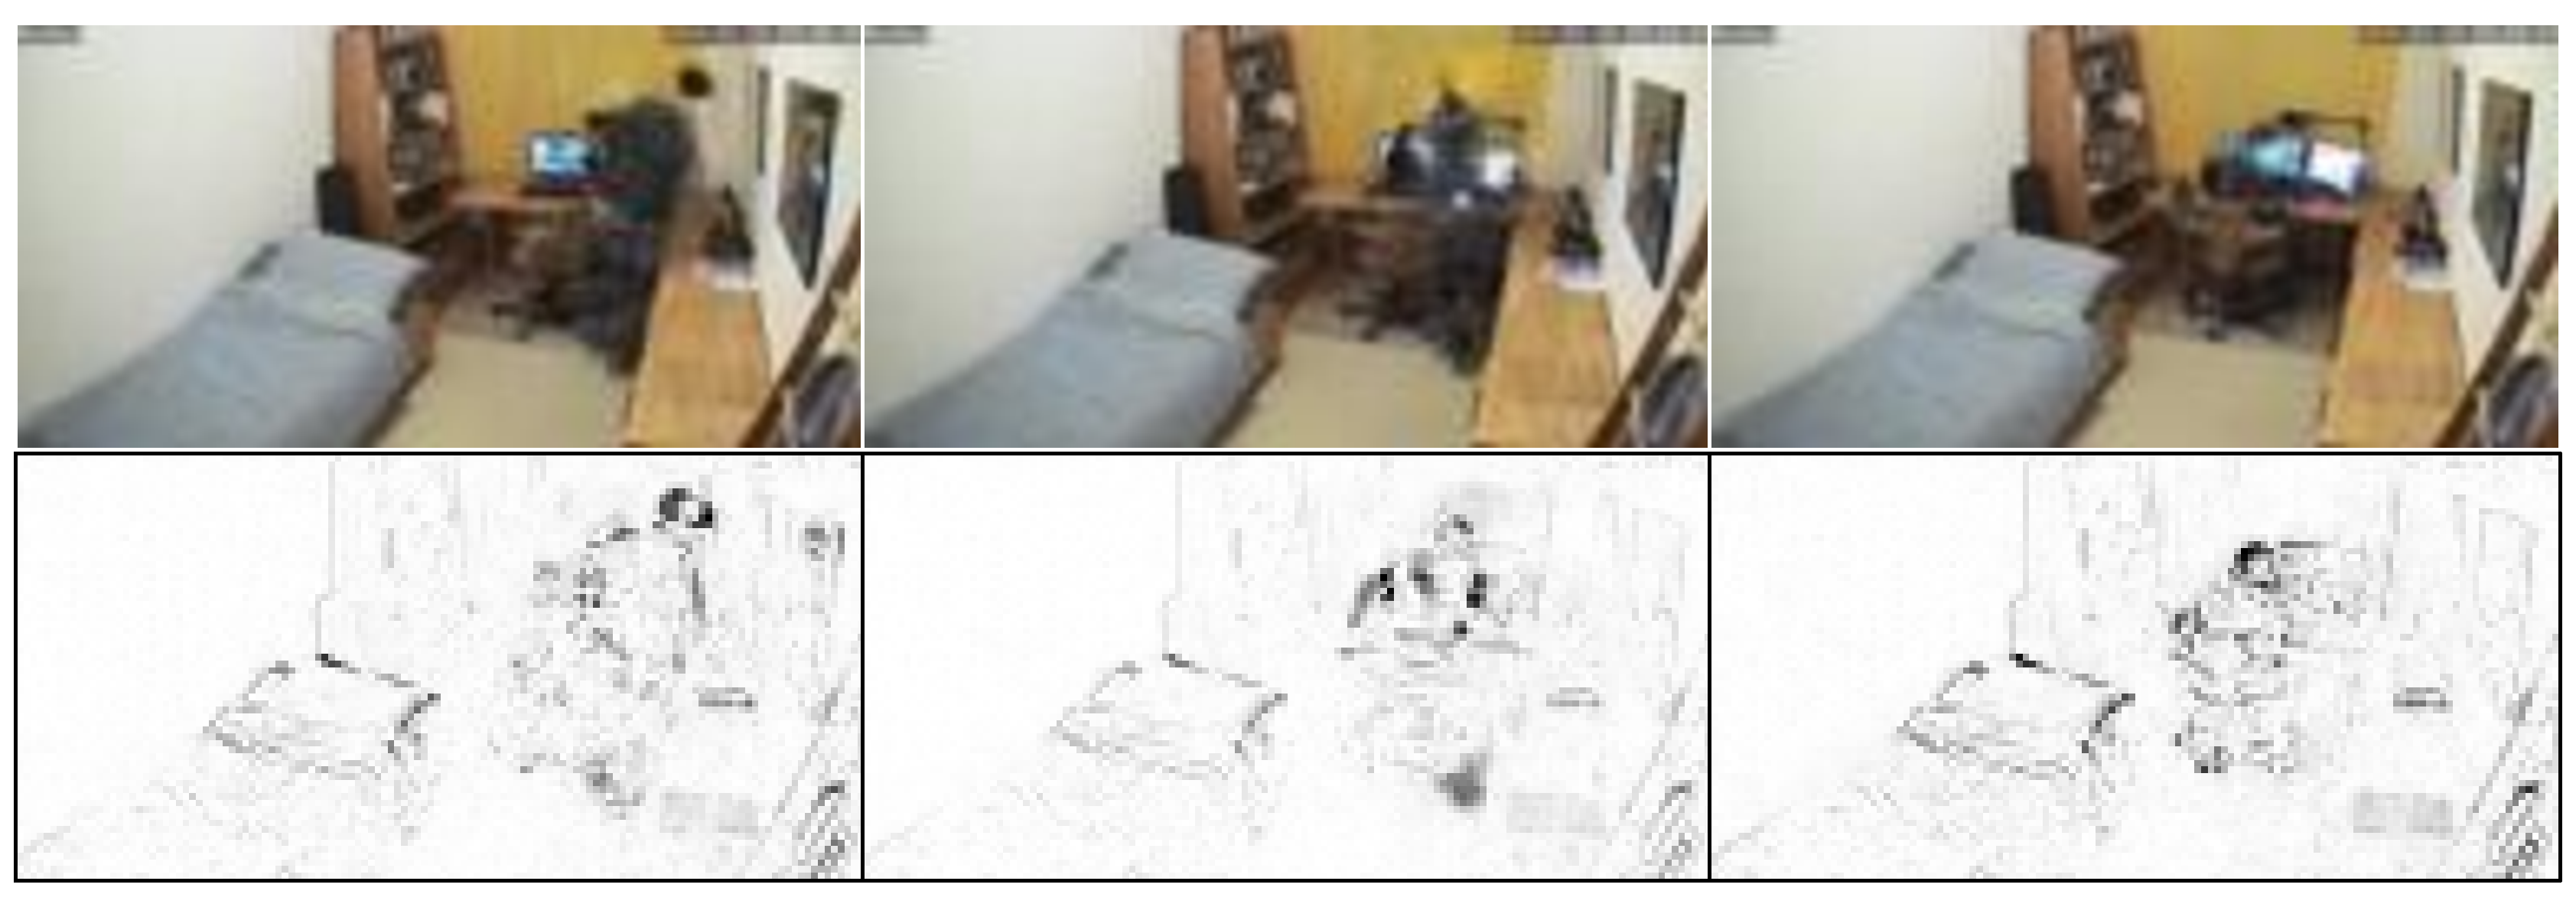
\includegraphics[width=0.9\textwidth]{graphics/eval/cvgan_2/qual_prediction/cvgan_2_dfilter-16_ddropout-0.3_lambda-10_batchsize-8_learningrate-0.0002_epochs-0050/normal.pdf}
		\caption{cf=16, dr=0.3, $\lambda$=10, bs=8, lr=2e-4}
		\label{subfig:bs8-pred-n}
	\end{subfigure}
	
	\caption[Prediction error heat maps for normal frames predicted by C-VGANs.]{Comparison between the actual next frames (a) and predictions by two differently configured C-VGAN models, further illustrated and dissected as heat maps of the pixel-wise mean absolute error. Note that the overall prediction error for these frames should be minimal, as they only contain assumed normal object patterns (see Section \ref{subsec:dataset_properties}).}
	\label{fig:cvgan_prediction_normal}
\end{figure}

\begin{figure}
  \centering

	\begin{subfigure}{\textwidth}
		\centering
		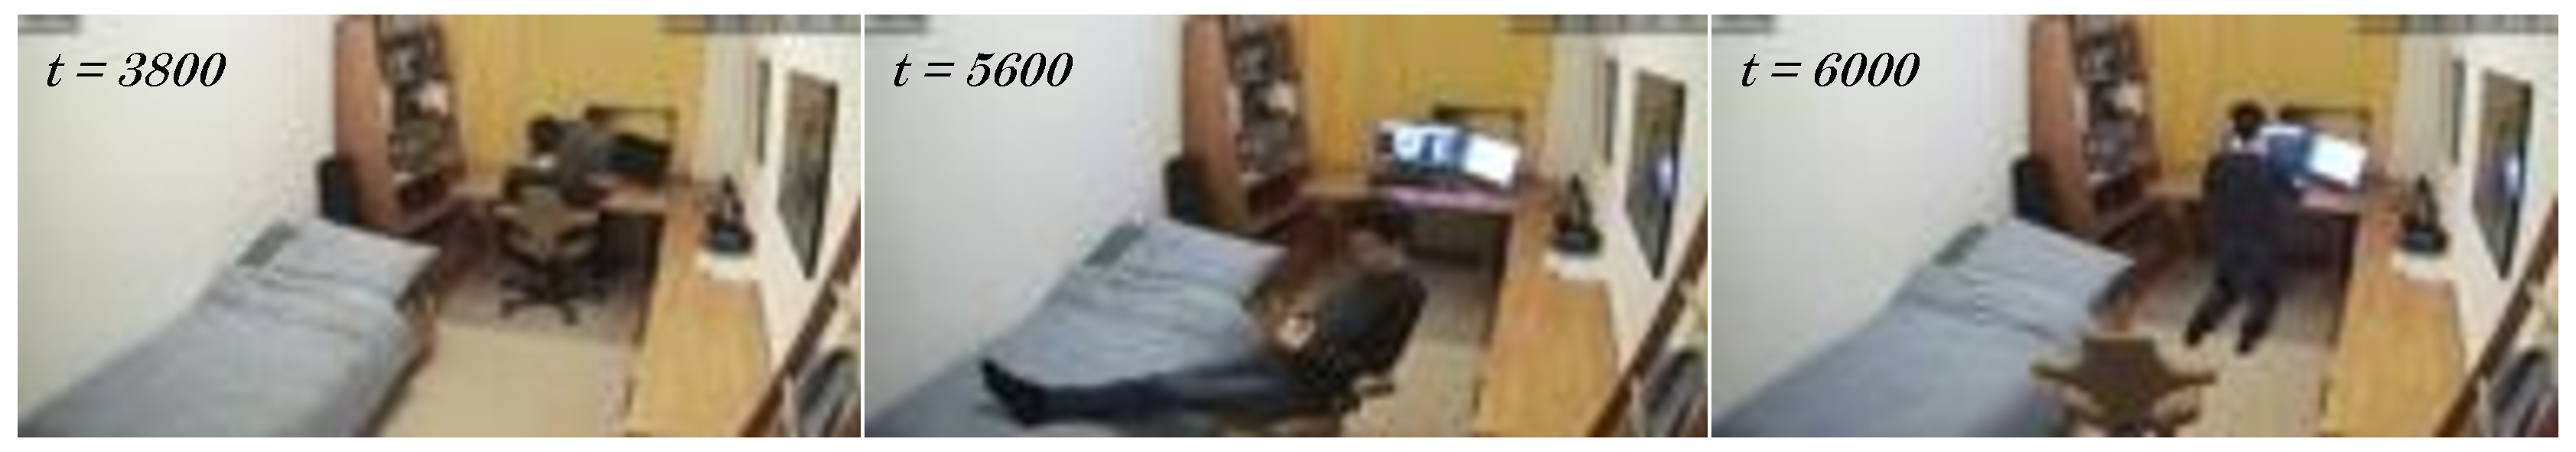
\includegraphics[width=0.9\textwidth]{graphics/eval/cvgan_2/qual_prediction/real/anomalous.pdf}
	  \caption{Actual next frames.}
	  \label{subfig:cvgan_prediction_anomalous}
	\end{subfigure}
	
  \begin{subfigure}{\textwidth}
	  \centering
		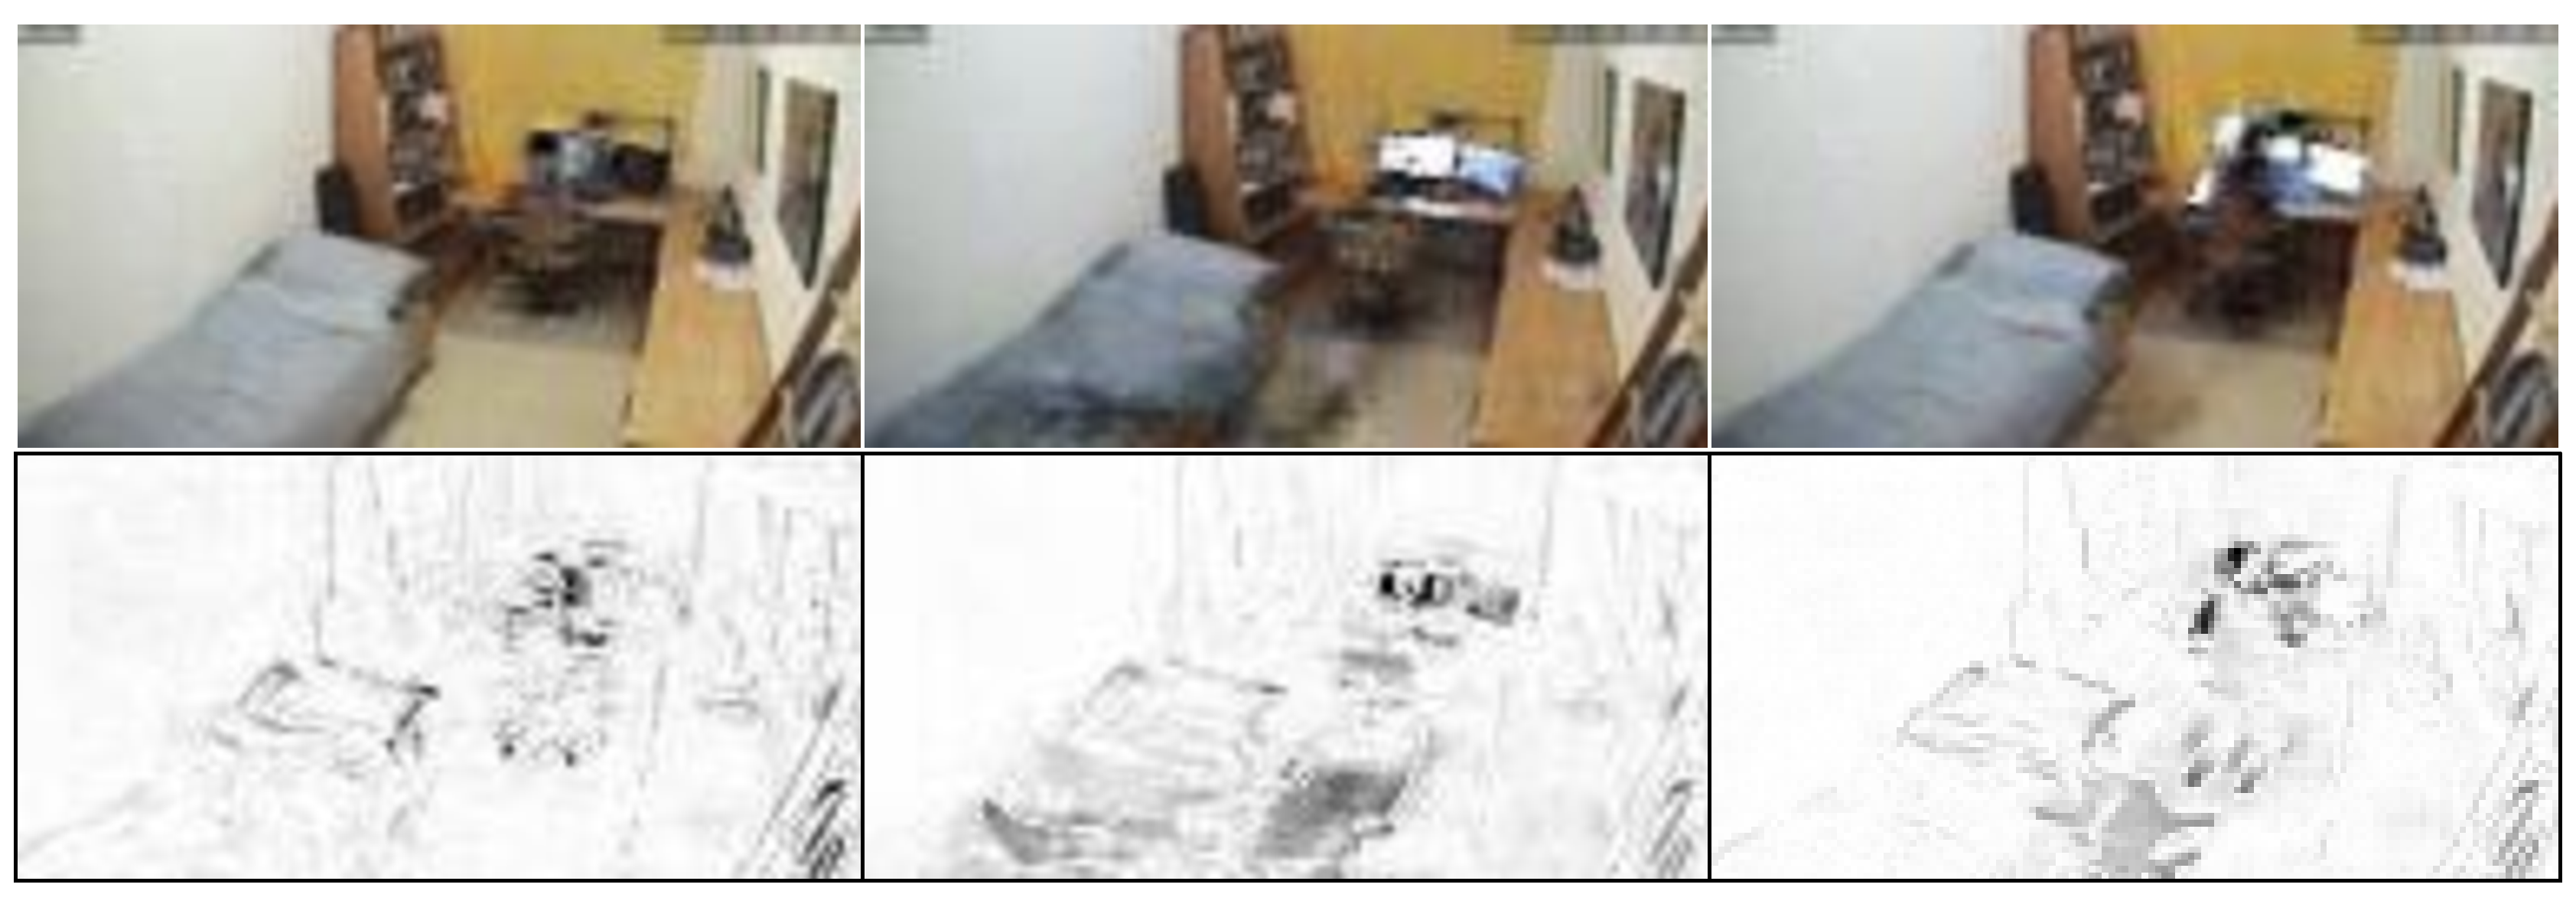
\includegraphics[width=0.9\textwidth]{graphics/eval/cvgan_2/qual_prediction/cvgan_2_dfilter-16_ddropout-0.3_lambda-10_batchsize-128_learningrate-0.000282842712474619_epochs-0050/anomalous.pdf}
		\caption{cf=16, dr=0.3, $\lambda$=10, bs=128, lr=2.8e-4}
		\label{subfig:bs128-pred-a}
	\end{subfigure}	
	
	\begin{subfigure}{\textwidth}
	  \centering
		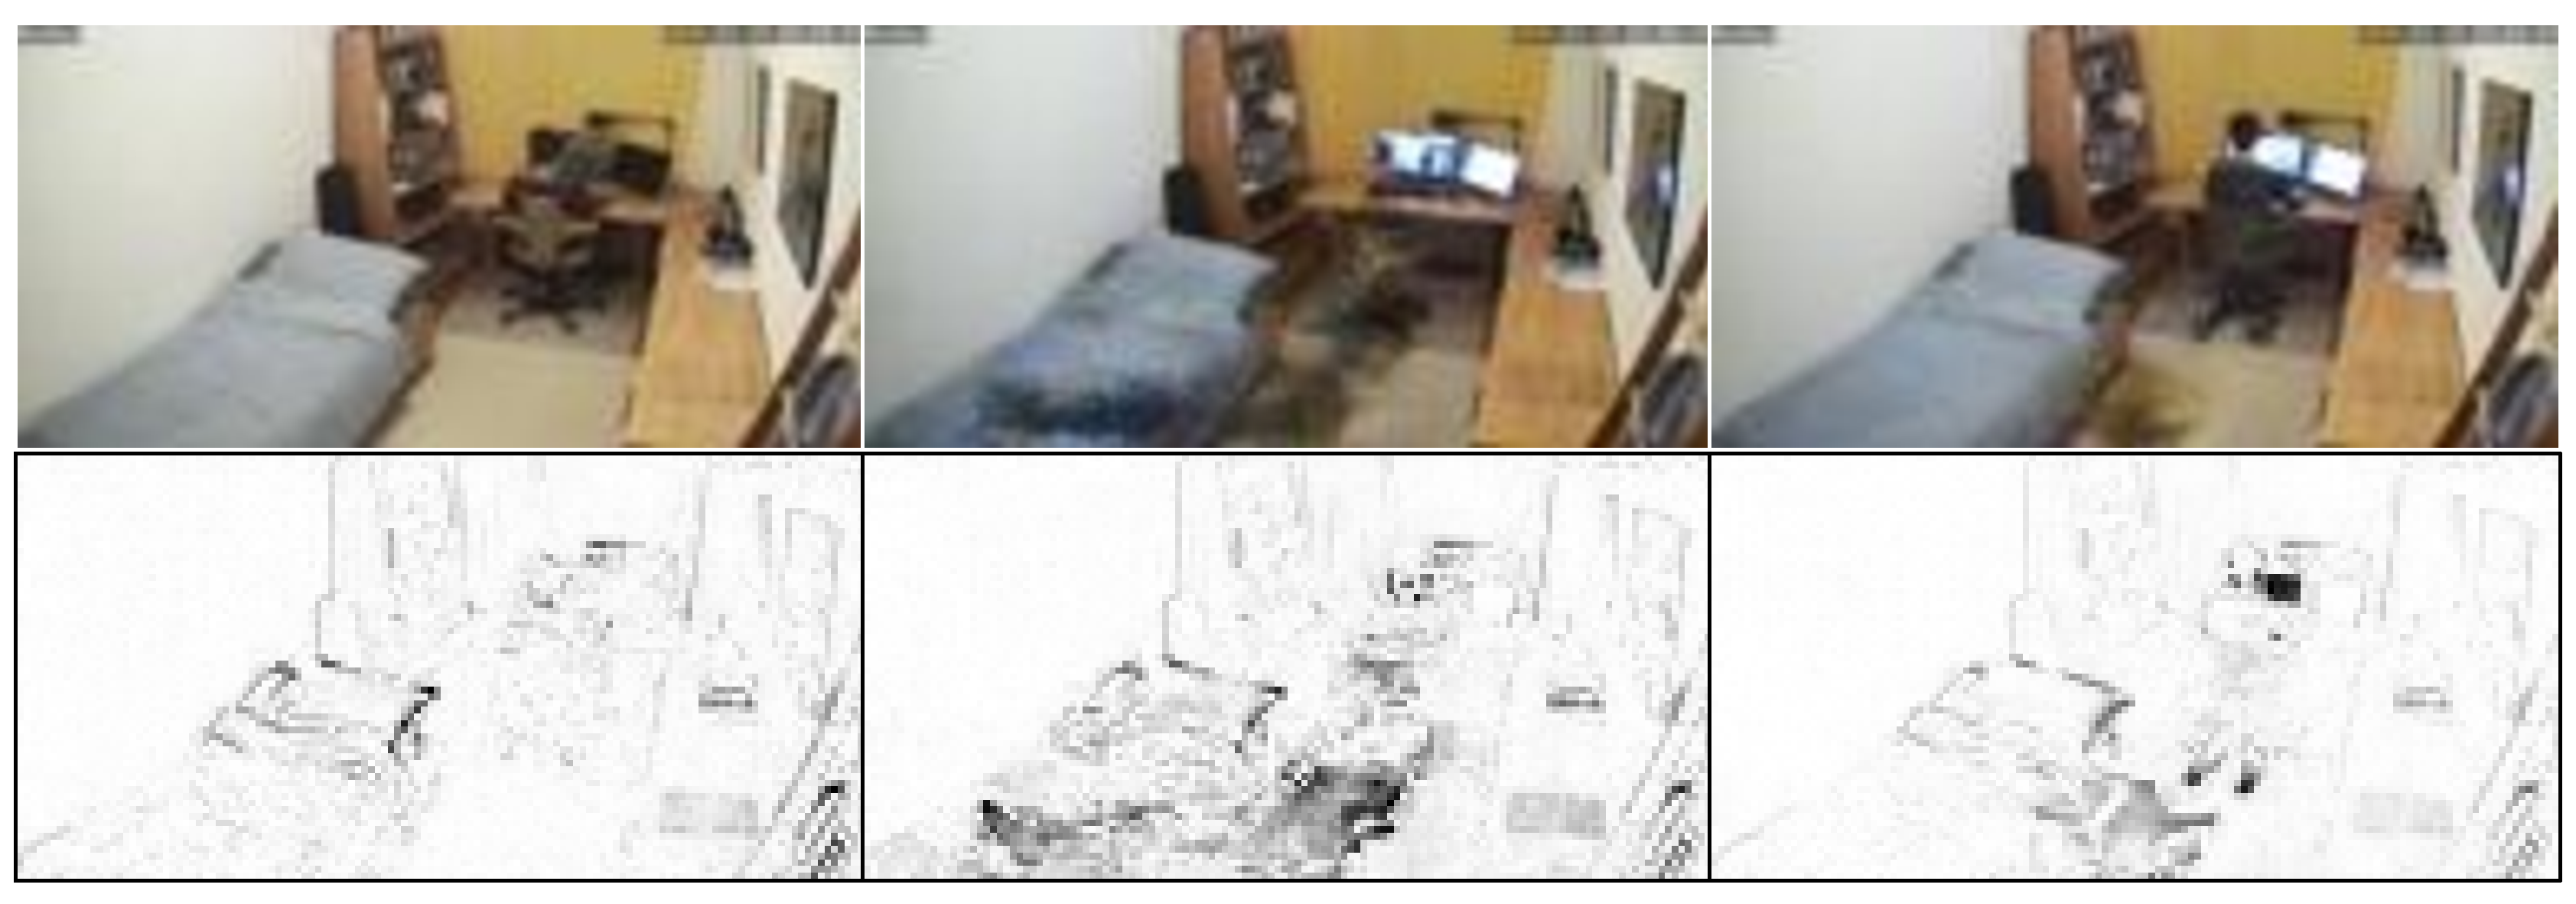
\includegraphics[width=0.9\textwidth]{graphics/eval/cvgan_2/qual_prediction/cvgan_2_dfilter-16_ddropout-0.3_lambda-10_batchsize-8_learningrate-0.0002_epochs-0050/anomalous.pdf}
		\caption{cf=16, dr=0.3, $\lambda$=10, bs=8, lr=2e-4}
		\label{subfig:bs8-pred-a}
	\end{subfigure}
	
	\caption[Prediction error heat maps for anomalous frames predicted by C-VGANs.]{Comparison between the actual next frames (a) and predictions by two differently configured C-VGAN models, further illustrated and dissected as heat maps of the pixel-wise mean absolute error. Note that these frames are considered anomalous in nature (see Section \ref{subsec:dataset_properties}), so for the purpose of IFTM, the models must be unable to predict these as accurately as normal frames.}
		\label{fig:cvgan_prediction_anomalous}
\end{figure}

The benefit of smaller batches during training becomes even more apparent, when evaluating some of the models based on their prediction quality on the evaluation data set. In Figure \ref{fig:cvgan_prediction_normal}, one can see three frames and how they were predicted by two configurations using different batch sizes. These frames are part of a larger event in which the person moves towards the desk and sits down. One can see how a larger batch size is unable to model any of the motion dynamics properly, trying to hallucinate a sitting person at the desk in the second and third depicted frame, but even failing to do that. A batch size of $8$ on the other hand manages to model the initial movement, before failing to accurately model the sitting down motion pattern. It can be assumed that the model lacked many diverse observations in which these object patterns occur, so it naturally struggles to make reconstructions and predictions for such rare events. Yet the heat map shows that the object with the motion pattern is not driving the over all prediction error for C-VGAN with bs=$8$, not unlike for a batch size of $128$. 

When giving both configurations anomalous events from the evaluation data set however, one notices that a smaller batch size also helps with the generalization and prediction of these anomalous frames, which is detrimental to our use case: In the first frame of Figure \ref{fig:cvgan_prediction_anomalous}, the computer displays are turned off while the person sits at the desk for a while --- a collective anomaly, but besides hallucinations of a bit of light on one of the displays for the model that was trained using the larger batch size, there are not any noticeable prediction errors showing on the heat map for that event. On the other hand, when anomalous object patterns are less local and occur in larger portions of the scene, both models successfully fail to model them properly. As seen in the heat maps of the second and third example, their errors are mostly the same, with the generator being able to partially omit the person sitting in the middle of the room.

Nonetheless, the first anomalous example in the figure is a symptom of a larger problem when training video generation models not only for prediction, but to only be able to model the normal state of the system, while being unable to make predictions during anomalous events. For the latter, our models seem to be able to generalize the future well enough, so that this particular series of anomalous frames can be accurately predicted. And these predictions even have a smaller error than some of the normal examples depicted in Figure \ref{fig:cvgan_prediction_normal}. Then, there are also prediction errors occurring in unexpected places: The outlines of the pillows on the bed, but also the shelf in the background, some papers on the lowboard, and the ladder in the right foreground are visible in all the depicted error heat maps, both anomalous frames and normal. This is an indicator for an occurrence of output collapse, because the models, as explained in our methodology in the previous section, are only trained with $6$ days of data. This in the worst case, gives the models only $6$ different positions for the pillows, as the bed is only made once per day. Unlike with various other object patterns and for the person interacting with the room, any new position of these pillows either has to be reconstructed or is collapsed into one of the known object patterns. The same is the case for the papers on the lowboard and the other examples listed above, creating a constant noise of falsely predicted normal object patterns in each frame that is not from the training split. Note that these errors can be safely ignored, when using C-VGAN for next-frame predictions, as these errors are barely noticeable by a human. But when using such a model for IFTM and VAD, these static errors for normal object patterns in a scene will skew with the classification results, as it gives all incoming frames a higher anomaly score no matter the true label. This challenge and how it can be solved to improve on the quality of our anomaly detection approach for video, will be discussed after the VAD evaluation results have been presented in the following section.



% Anomaly Detection Evaluation
\section{Anomaly Detection for Video using IFTM} \label{sec:vad_eval}

Loading C-VGAN models for next-frame video prediction into the adapted IFTM framework presented in Section \ref{sec:vad}, the ADS can then be evaluated on its performance for VAD. As mentioned throughout the previous chapter, the modified version of IFTM has no additional hyperparameters that need tuning: The identity function (IF) is the fully trained prediction generator model of C-VGAN loaded from disk, while the threshold model (TM) can be computed using the training data set, the IF, and the prediction error function. Hence in this Section, C-VGAN generators that were evaluated in the prior section are taken as they are. To assess IFTM with different underlying prediction models, quantitative metrics were chosen as the main tool for evaluation. These are provided first, with an explanation of their meaning. The resulting anomaly detection metrics for the different IFTM configurations is then presented afterwards.


% Anomaly Detection Evaluation Methods
\subsection{Evaluation Method} \label{subsec:vad_eval_method} % 3 Pages

\paragraph{Confusion Matrix and Derived Metrics}

\begin{table}
	\centering
	\begin{tabular}{| c | c | c | c |}
	\toprule
	\multicolumn{2}{| c |}{\multirow{2}{*}{}} 	  & \multicolumn{2}{ c |}{\textit{\textbf{Actual}}} \\
	\cmidrule{3-4}
	\multicolumn{2}{| c |}{} 						          & \textbf{Anomaly} & \textbf{Normal} \\
	\midrule
	\multirow[c]{2}{*}{\textit{\textbf{Predicted}}}& \textbf{Anomaly} 	& True Positive (TP)  & False Positive (FP)	\\
	\cmidrule{2-4}
												  & \textbf{Normal} 	& False Negative (FN) & True Negative (TN)	\\
	\bottomrule
	\end{tabular}
	\caption[Confusion matrix for anomaly detection evaluation.]{Binary confusion matrix for anomaly detection evaluation.}
	\label{tab:confusion_matrix}
\end{table}

Our adapted version of IFTM labels every frame in a video stream in binary fashion (0=normal and 1=anomalous). And, as explained in Section \ref{subsec:framework_iftm} and \ref{subsec:postprocessing}, these predicted labels can then logged and be used to quantitatively evaluate different model configurations. Using our labeled evaluation data set presented in detail in Section \ref{sec:dataset}, we can compare the true label of each frame to the one predicted by a model. Doing this over the entire data set and aggregating the results, a confusion matrix for all existing samples and their classes can be constructed, as shown in Table \ref{tab:confusion_matrix}: A special kind of contingency table, the rows of the matrix represent the instances in the predicted classes, while the columns are the instances in the actual classes. Given it is a binary matrix, there are four outcomes: If an anomalous frame was labeled as an anomaly, it would count as a true positive, but if it was predicted to be normal, it would be a false negative, i.e. an omitted anomaly. Vice versa, if a normal frame was classified as an anomaly, it would be a false positive --- a false alarm. A true negative would be the same frame labeled as normal.

\begin{table}
	\centering
	\begin{tabular}{ | L{4.7cm} | l |}
	\toprule
	\textbf{Metric} & \textbf{Derivation from Confusion Matrix} \\
	\midrule
	True Positive Rate \quad \quad 
	(Recall, Sensitivity) & $TPR = \frac{TP}{TP + FN} = 1 - FNR$ \\[1ex]  %recall = tp / (tp + fn)
	True Negative Rate 
	(Specificity)  & $TNR = \frac{TN}{TN + FP} = 1 - FPR$ \\[1ex]  %tnr = tn / (tn + fp)
	Positive Predictive Value 
	(Precision)    & $PPV = \frac{TP}{TP + FP}$ 	        \\[1ex]  %precision = tp / (tp + fp)
	Negative Predictive Value
                 & $NPV = \frac{TN}{TN + FN}$ 	        \\[1ex]  %npv = tn / (tn + fn)
	False Positive Rate \quad \quad 
	(Fall-Out)     & $FPR = \frac{FP}{FP + TN} = 1 - TNR$ \\[1ex]  %fpr = fp / (fp + tn)
	False Negative Rate \quad \quad 
	 (Miss Rate)   & $FNR = \frac{FN}{FN + TP} = 1 - TPR$ \\[1ex]  %fnr = fn / (fn + tp)
	Accuracy       & $Acc = \frac{TP + TN}{TP + TN + FP + FN} = \frac{TP + TN}{total}$ \\[1ex]  %accuracy = (tp + tn) / self.total
	F-Measure      & $F_1 = \frac{2 \cdot TP}{2 \cdot TP + FP + TN} = \frac{2}{TPR^{-1}+PPV^{-1}}$ 	\\[1ex]  %f1 = 2 * tp / (2 * tp + fp + fn)
	\bottomrule
	\end{tabular}
	\caption[Anomaly detection evaluation metrics.]{Anomaly detection evaluation metrics, derived from the binary confusion matrix. Often used aliases for the metrics are given in parenthesis.}
	\label{tab:eval_metrics}
\end{table}

Using the aggregated counts of each outcome, one can derive many commonly used evaluation metrics from it. For the quantitative evaluation of IFTM for VAD, the eight metrics presented in Table \ref{tab:eval_metrics} were selected: First, it is important to evaluate how many of the actual normal and anomalous samples were correctly predicted by the detection model. Recall and specificity represent these two rates. Their direct counterparts, the rates anomalies and normal data points are labeled incorrectly are redundant but helpful to inspect the rate of false alarms and omitted anomalies directly. This is especially useful in case a model is very sensitive: Detecting nearly every frame as an anomaly would result in both a high recall and a high false alarm rate (fall-out). Next, positive and negative predictive value represent how many of the instances of their predicted respective classes actually belong to their class. But these two metrics can also be deceiving, especially in unbalanced data sets. For example, roughly $30\%$ of our evaluation data set are anomalies, as presented in detail in Section \ref{sec:dataset}. Labeling all of the data set's samples as normal would result in a fairly high negative predictive value ($70\%$). At the same time, a high positive predictive value can be achieved by exclusively labeling a few actual anomalous data points as anomalies, while still classifying most actual anomalies incorrectly. 

There are metrics which try to aggregate the information of the confusion matrix further: Accuracy depicts the overall rate of correct predictions. Although it has similar issues as the metrics above if the data set is unbalanced --- labeling one class mostly correctly while ignoring the other can still achieve a high accuracy under those circumstances, it can still be used as an additional indicator for a good anomaly detection model. In addition, we chose the F-measure as our last evaluation metric, which combines recall and precision into a single value using the harmonic mean. This metric would be lower in case a model classified all samples as anomalies for example, resulting in a high recall, but a low precision. However the metric lacks meaningful information on the true negatives. In the end there is no catch-all metric for quantitative anomaly detection evaluation, and the combination of the selected metrics needs to be utilized to assess the models during the presentation of the results in the following section.

\paragraph{Prediction Error over Time}
Although for anomaly detection evaluation, the quantitative metrics are sufficient indicators for the overall performance of a given model, the metrics are computed over the model's performance on the entire evaluation data set. But this data set is not homogeneous, nor is every frame created equal: As analyzed in Section \ref{subsec:dataset_properties}, normal and anomalous frames occur in clustered events, respectively. Some of these events rely heavily on motion dynamics, while others have static contextual information that is sufficient enough to discriminate normal from anomalous properties. A simple motion detector might be able to classify some of the more static events correctly --- both normal and anomalous ones, but at the same time it would classify all events containing motion dynamics as anomalies. To identify such root causes and other kinds of quirks in the models' preference in properties to discriminate the classes, one needs to drill-down and inspect the performance on a smaller scale. Granted it could be of interest to split the evaluation data set further into its events or specific event categories to evaluate different performance aspects of an anomaly detection model, the resulting number of quantitative metrics would blow up and evaluation of multiple configurations would be unfeasible. 

Thus a different approach was chosen: With IFTM having both a static prediction model and threshold, the prediction errors for each frame in the video stream can be arranged and analyzed as a time series. Evaluation in that case is done qualitatively, assessing the prediction error over time in the video stream. This approach can also be also used to evaluate where and how false alarms and omissions occur and with which events IFTM with C-VGAN struggles. Lastly it is to note, that failure to classify certain events does not necessarily mean that the model is of bad quality: If for example omissions of anomalies occur throughout the evaluation of different C-VGAN configurations, the underlying video generation model might be able to generalize well enough to make sufficient predictions for certain anomalous frames. And, as the frames of the evaluation data set were labeled by a human, this could be an indicator that some of the created events are too similar to normal ones --- and vice versa, when it comes to their features that are extracted by the prediction model. In other cases, the evaluation of the prediction errors can also help with the assessment of the threshold model and whether its static modeling based on the training data accurately reflects the mapping of normal and anomalous frames' predictions errors to their binary classes. 

This kind of assessment has some overlap with the second half of the qualitative evaluation method for C-VGAN in Section \ref{par:cvgan_eval_method_qual}, as both methods inspect the prediction errors of the evaluation data set. But while the former focuses purely on the video prediction quality on unknown data and how it performs on both normal and anomalous videos, in context of IFTM, the overall prediction error for each frame is analyzed in combination with the threshold. Meaning, fluctuations in the model's prediction quality are not of interest as long as the error falls below threshold $T$ for normal samples. Yet this overlap that results in some correlation of the results will be discussed in Section \ref{sec:discussion}, after the results of IFTM for VAD have been presented.


% Anomaly Detection Results
\subsection{Results} \label{subsec:vad_results} % 5 Pages

\paragraph{Evaluation Metrics}

\begin{table}
	\centering
	\begin{tabular}{ | c | c | c | c | c | r | r | r | r | r | r |}
	\toprule
	\multicolumn{5}{| c |}{\textbf{C-VGAN Configuration}} & \multicolumn{1}{c |}{\multirow[c]{2}{*}{\textbf{Accuracy}}} & \multicolumn{1}{c |}{\multirow[c]{2}{*}{\textbf{Precision}}} & \multicolumn{1}{c |}{\multirow[c]{2}{*}{\textbf{Recall}}} & \multicolumn{1}{c |}{\multirow[c]{2}{*}{\textbf{Fall-Out}}} & \multicolumn{1}{c |}{\multirow[c]{2}{*}{\textbf{F-Measure}}} \\ \cmidrule{1-5}
	$cf$ & $dr$ & $\lambda$ & $bs$ & $lr$ & & & & & \\
	\midrule
	\multirow[c]{11}{*}{$16$} & $0.0$ & $10$  & $64$ & $2.0$\text{e-}$4$ 
	    & $74.48\%$ & $69.49\%$ & $29.27\%$ & $5.65\%$ & $41.19\%$ \\ \cline{2-5}
	& \multirow[c]{10}{*}{$0.3$} & $5$ & $64$ & $2.0$\text{e-}$4$ 
	    & $74.36\%$ & $64.01\%$ & $36.60\%$ & $9.04\%$ & $46.57\%$ \\
	& & $8$ & $64$ & $2.0$\text{e-}$4$ 
	    & $\mathbf{81.71\%}$ & $\mathbf{68.59\%}$ & $\mathbf{73.95\%}$ & $\mathbf{14.89\%}$ & $\mathbf{71.17\%}$ \\ \cline{3-5}
	& & \multirow[c]{6}{*}{$10$} & $8$ & $2.0$\text{e-}$4$ 
	    & $31.35\%$ & $30.79\%$ & $100.00\%$ & $98.84\%$ & $47.08\%$ \\
	& &      & $16$ & $2.0$\text{e-}$4$ 
	    & $34.83\%$ & $31.91\%$ & $100.00\%$ & $93.82\%$ & $48.38\%$ \\
	& &      & $32$ & $2.0$\text{e-}$4$ 
	    & $49.50\%$ & $37.54\%$ & $98.48\%$ & $72.03\%$ & $54.36\%$ \\
	& &      & $64$ & $2.0$\text{e-}$4$ 
	    & $75.67\%$ & $56.25\%$ & $91.43\%$ & $31.26\%$ & $69.65\%$ \\
	& &      & $128$ & $2.8$\text{e-}$4$ 
	    & $\mathbf{82.33\%}$ & $\mathbf{71.70\%}$ & $\mathbf{69.62\%}$ & $\mathbf{12.08\%}$ & $\mathbf{70.65\%}$ \\
	& &      & $256$ & $4.0$\text{e-}$4$ 
	    & $70.02\%$ & $51.42\%$ & $33.10\%$ & $13.75\%$ & $40.27\%$ \\ \cline{3-5}
	& & $14$ & $64$ & $2.0$\text{e-}$4$ 
	    & $75.85\%$ & $60.53\%$ & $60.14\%$ & $17.24\%$ & $60.33\%$ \\
	& & $20$ & $64$ & $2.0$\text{e-}$4$ 
	    & $75.18\%$ & $57.40\%$ & $72.59\%$ & $23.68\%$ & $64.11\%$ \\ \cline{1-5}
	$32$ & $0.0$ & $10$ & $64$ & $2.0$\text{e-}$4$ 
	    & $73.25\%$ & $65.67\%$ & $25.97\%$ & $5.97\%$ & $37.23\%$ \\
	\bottomrule
	\end{tabular}
	\caption[IFTM anomaly detection evaluation results.]{Anomaly detection evaluation results for IFTM using different C-VGAN models as a forecasting model (IF); to be considered best results written in bold. Note a differently configured and trained IF also affects the TM, as it has to be trained based on the IF's predictions on the training data set.}
	\label{tab:eval_metrics_results}
\end{table}

Table \ref{tab:eval_metrics_results} shows the performance of IFTM models using the different C-VGAN models presented in Section \ref{subsec:cvgan_results}. To not display redundant metrics that are the counter-probability of another one, the true and false negative rate are omitted in that table; as explained in the previous section they can be directly derived from the false and true positive rate (fall-out, recall), respectively. Matching some of the results of our C-VGAN evaluation, models in which the discriminator was not sufficiently impaired during training and the generator was not satisfactory in quality (cf=$32$; cf=$16$, dr=$0.0$), have both lower recall and fall-out metrics. This happens when IFTM is not sensitive enough and only detects the most anomalous events. All other frames' prediction errors are the same and thus are indistinguishable for the TM, which labels them all as normal. In addition, the trained C-VGAN models of these configurations from different training epochs were put into IFTM and the VAD systems were again evaluated. They all produced similar or worse results and were therefore discarded for further evaluation. Contrary to the presented results of C-VGAN in Section \ref{subsec:cvgan_results} and our expectations, the IFTM configurations using smaller batch sizes during the training of C-VGAN proved to be too sensitive. Labeling all but the most extreme outliers as normal, they have a very high recall and fall-out, which makes them useless for any form of VAD. With $\sim 30\%$ of frames being anomalies, the accuracy and precision default to the same value. On the other hand, when using higher batch sizes (bs=$128$) or increasing the degrees of freedom for the forecasting model ($\lambda$=$8$ instead of $10$) an accuracy of $>80\%$ and an F-score of $>70\%$, with the precision and recall also being around $70\%$, can be achieved. Which of the two is to be preferred depends on how costly false positives actually are; having a $25\%$ (relatively) higher fall-out with only a slight increase in recall requires disproportional more manual oversight to filter out false anomalies. For lower or even higher values of $bs$, the results are again worsening. The same is the case when further increasing or decreasing $\lambda$ --- the former action makes the model more sensitive to anomalies but also raises the false positive rate, while the latter decreases it, but at a cost of the recall.

Based on the results of the metrics shown above, we therefore recommend a default configuration of the reconstruction loss weight $\lambda$, a sufficiently impaired discriminator (cf=$16$, dr=$0.3$) and a higher batch size (bs=$128$) with a fitting higher learning rate (lr=$2.8$\text{e-}$4$).

\paragraph{Prediction Error vs Threshold}

\begin{figure}
  \centering
  
  \begin{subfigure}{\linewidth}
    \centering
		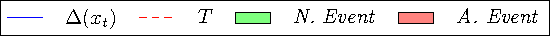
\includegraphics[width=0.5\linewidth]{{graphics/eval/iftm/errors/error_legend}.pdf}
	\end{subfigure}
	\vspace{0.01cm}

	\begin{subfigure}{\textwidth}
	  \centering
		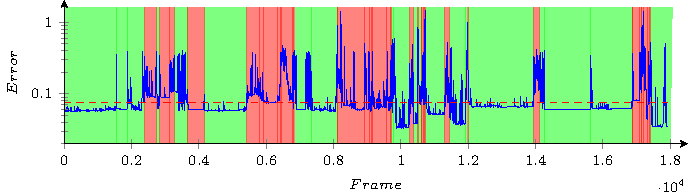
\includegraphics[width=\textwidth]{{graphics/eval/iftm/errors/cvgan_2_dfilter-16_ddropout-0.3_lambda-10_batchsize-128_learningrate-0.000282842712474619_epochs-0050_errorfn-mean_absolute_error_res}.pdf}
		\vspace{-0.7cm}
		\caption{cf=16, dr=0.3, $\lambda$=10, bs=128, lr=2.8e-4}
		\label{subfig:bs128-error-1}
	\end{subfigure}

	\begin{subfigure}{\textwidth}
	  \centering
		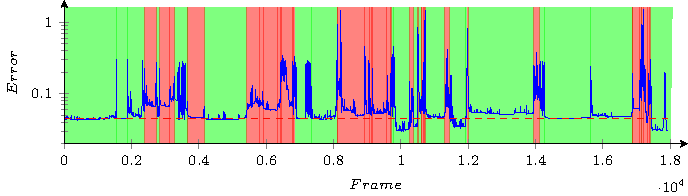
\includegraphics[width=\textwidth]{{graphics/eval/iftm/errors/cvgan_2_dfilter-16_ddropout-0.3_lambda-10_batchsize-32_learningrate-0.0002_epochs-0050_errorfn-mean_absolute_error_res}.pdf}
		\vspace{-0.7cm}
		\caption{cf=16, dr=0.3, $\lambda$=10, bs=32, lr=2e-4}
		\label{subfig:bs32-error-1}
	\end{subfigure}	
	
	\begin{subfigure}{\textwidth}
	  \centering
		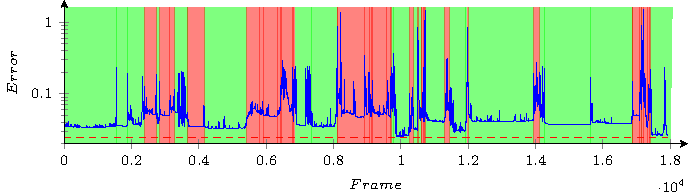
\includegraphics[width=\textwidth]{{graphics/eval/iftm/errors/cvgan_2_dfilter-16_ddropout-0.3_lambda-10_batchsize-8_learningrate-0.0002_epochs-0050_errorfn-mean_absolute_error_res}.pdf}
		\vspace{-0.7cm}
		\caption{cf=16, dr=0.3, $\lambda$=10, bs=8, lr=2e-4}
		\label{subfig:bs8-error-1}
	\end{subfigure}

	\caption[Prediction error of the underlying forecasting models of IFTM.]{Prediction error ($\Delta(x_t)$) for the evaluation data set of IFTM using different C-VGAN models as a forecasting model (IF). An error greater than threshold ($T$) is classified as an anomaly. The actual normal and anomalous events of the labeled data set are represented by the colored background (see Section \ref{subsec:dataset_properties}).}
	\label{fig:if_error_1}
\end{figure}

Since the quantitative results are not only counter intuitive, but also not desired --- our best configuration for VAD having an underlying forecasting model that failed our qualitative C-VGAN evaluation due to object pattern omissions and hallucinations, the results when using different batch sizes during training need to be verified. In Figure \ref{fig:if_error_1} three different IFs' prediction errors over the entire evaluation data set and their respective TMs are displayed. Underlaid in green and red respectively, the true labels are shown, with red and green lines being separations between different events, as further explained in detail in Section \ref{subsec:dataset_properties}, where the data set was dissected into each event. First it is of interest, how every graph is similar to one another, with the only notable difference being the overall prediction error. For the first in Figure \ref{subfig:bs128-error-1}, having the best quantitative results before, the errors are far higher (the y-axis is a log scale) compared to the other displayed configurations. Threshold $T$ in that case is able to separate the two classes except for a few outliers over the entire series and an anomalous event at $t=[3673,4169]$. This event, that was already mentioned in the results of C-VGAN will be discussed in the following section further, was misclassified by all configurations except the very sensitive models, that mislabeled every normal event instead. There is also an anomalous event around $t=9000$, which was partially falsely labeled.

Compared to the quantitative results, lower batch sizes ($bs$) during training actually improved the prediction quality of the forecasting model, resulting in a overall lower prediction error. This mirrors our qualitative results of C-VGAN, with these models being among the best in terms of video quality, minimal hallucinations, omissions, and object collapsing. They also did better for scenes involving motion dynamics, while configurations with higher batch sizes sometimes omitted dynamic object patterns completely from the scene. But the prediction error on unknown normal frames is still higher than the threshold $T$. Disproportionately so with lower batch sizes. This is the case, because, as explained in Section \ref{sec:vad}, the TM is computed based on the mean prediction error on the training data set and the standard deviation. And, when having a model that has an overall better prediction quality, the training error might usually also decrease but at a different pace than the error on unknown data. This can create a TM that is far more sensitive than in other configurations. Note that this phenomenon is not some kind of overfitting, since generalization also improves. The same scenario occurs when one increases or decreases the number of training epochs of the underlying C-VGAN model. The former causes a more sensitive threshold but a lower prediction error on the evaluation data set, which in return increase both recall and fall-out. Meanwhile the latter decreases the sensitivity of IFTM by having a too high threshold for the prediction errors, which causes omissions and a high false negative rate.



% Discussion of the Results
\section{Discussion} \label{sec:discussion} % 3-4 Pages

\begin{figure}
  \centering
  
  \begin{subfigure}{\textwidth}
	  \centering
	  \begin{tabular}{ | L{2.5cm} | r | r | r | r | r | r |}
	  \toprule
	  \textbf{Threshold}  & \multicolumn{1}{c |}{\textbf{Accuracy}} & \multicolumn{1}{c |}{\textbf{Precision}} & \multicolumn{1}{c |}{\textbf{Recall}} & \multicolumn{1}{c |}{\textbf{Fall-Out}} & \multicolumn{1}{c |}{\textbf{F-Measure}} \\
	  \midrule
	  $T_0\approx 2.434\text{e-}2$ & $31.35\%$ & $30.79\%$ & $100.00\%$ & $98.84\%$ & $47.08\%$ \\
	  $T_1\approx 4.865\text{e-}2$ & $87.13\%$ & $78.07\%$ & $80.46\%$  & $9.94\%$  & $79.25\%$ \\
	  \bottomrule
	  \end{tabular}
	  \caption{Anomaly detection evaluation metrics.}
		\label{subfig:iftm_alt_threshold_metrics}
  \end{subfigure}
  \vspace{0.1cm}
  
  \begin{subfigure}{\linewidth}
    \centering
		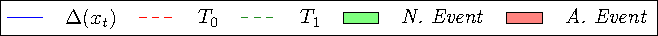
\includegraphics[width=0.6\linewidth]{{graphics/eval/iftm/altThreshold/altThreshold_legend}.pdf}
	\end{subfigure}

	\begin{subfigure}{\textwidth}
	  \centering
		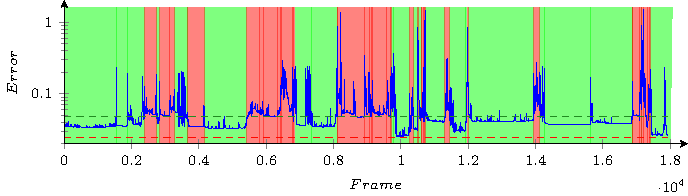
\includegraphics[width=\textwidth]{{graphics/eval/iftm/altThreshold/altThreshold}.pdf}
		\vspace{-0.7cm}
		\caption{Prediction error ($\Delta(x_t)$) underlaid by the labeled events.}
		\label{subfig:iftm_alt_threshold_error}
	\end{subfigure}
	
	\caption[Comparison between differently trained thresholds using the same IF.]{Comparison between threshold $T_0$ trained using the training split of the training data set and $T_1$. The latter was computed using the prediction errors of the IF on the validation and test split of the training data set; these two splits while mostly containing normal data are unknown to the IF. The IF for both TMs is the same (cf=16, dr=0.3, $\lambda$=10, bs=8, lr=2e-4).}
	\label{fig:iftm_alt_threshold}
\end{figure}

First, when analyzing and discussing the results from the previous sections, it is to note that our recommended configuration of C-VGAN used in our modified IFTM framework and trained using $50$ epochs, is not ideal. When using a forecasting model as an IF the forecasting model should be able to model normal observations and make good predictions based on them. Therefore, a prediction model that performs this task better than another, should be more suitable as an IF. This is not the case here: As shown in Section \ref{subsec:cvgan_results} during the presentation of the results for next-frame forecasting, models trained using smaller batch sizes, were generally more suitable to predict normal frames, including frames which heavily featured rare but normal motion dynamics. In comparison, our recommended configuration of C-VGAN for IFTM was unable to model these motion patterns, collapsing them into static scenes. But, because this happens for both training and evaluation data set equally, the results prove that a TM can still be found that is able to separate the two classes, unlike for C-VGAN configurations that are better in prediction quality. 

This behavior of different configurations for IFTM can be explained however, when reviewing the error heat maps of some of the made predictions on the evaluation data set (Figure \ref{fig:cvgan_prediction_normal} and \ref{fig:cvgan_prediction_anomalous}): As was presented in the results for C-VGAN, there is a somewhat constant source of prediction errors from failure to reconstruct static but normal object patterns accurately in every scene. For example, collapsing slight but unknown variations of the position of pillows on the bed into ones witnessed during training. This is a form of prediction error that may be unnoticeable by a human, but when computing the absolute error between actual and predicted next-frame in IFTM, these errors influence the frame-wise error and thus their classification. And, the better a model is able to predict other parts of a scene, such as motion patterns (e.g. a walking person), the more these constant errors influence the overall anomaly score. This is also noticeable in the heat maps, since these static errors have a darker shade, i.e. relatively higher error to the maximum error of the frame, when comparing the C-VGAN configuration trained with batch size $8$ versus our recommended one for IFTM (bs=$128$). Contrary to that, these small but constant errors do not appear when running predictions on the training data set, because the prediction errors for these static normal object patterns do not occur. Therefore threshold $T$ that is computed by the TM is only reflective of the prediction error for the known training split of the training data set, but not for unknown data, making it too sensitive for certain C-VGAN configurations. This can be verified by re-training the TM not on the known training-split, but on the validation and test split of the training data; see Section \ref{subsec:cvgan_eval_method} for information on these splits. In this case, the constant prediction errors from static but normal object patterns also arise during the training of the TM and thus influence it. The resulting threshold $T_1$ for a configuration using a batch size of $8$ can be seen in Figure \ref{fig:iftm_alt_threshold}, compared to the original $T_0$. Note this new threshold, although the training data set might differ slightly in its normal observations from the ones found in the evaluation data set, is able to perform much better in separating the prediction error values for normal and anomalous frames. The anomaly detection evaluation metrics in Figure \ref{subfig:iftm_alt_threshold_metrics} reflect this, outperforming the oversensitive IFTM using the same underlying C-VGAN prediction model in every metric, but also the IFTM recommended by us from the previous results.

Besides that, there is still one anomalous event, whose collective prediction errors fall below $T_1$. At $t=[3673,4169]$, which was already mentioned during the qualitative evaluation of C-VGAN (see Figure \ref{fig:cvgan_prediction_anomalous} from that section). There it was found out, that most video prediction models generalize well enough to reconstruct and predict turned off computer displays, while the person sitting at the desk is pretending to work for several minutes. This is challenging to fix, because this state does indeed exist and is normal, yet only if it occurs for a few frames and not for longer. Meanwhile the IF only makes predictions based on $7$ frames from the past, without having further memory, which makes it unsuitable to detect such a collective anomaly. This could be solved by modifying the video generation model with some sort of recurrent component, such as LSTM \cite{hochreiter1997long} or a convolutional version of thereof \cite{shi2015convolutional}, that is able to capture more of the temporal information across frames in the video stream.

Finally, in the prediction error time series shown in Figure \ref{subfig:iftm_alt_threshold_error}, one can also see normal events in which the prediction errors are more stable than during others. The latter being the case during event $t=[1558,1876]$ and $t=[14270,15641]$, both of which are events without any motion patterns; the room is empty and the scene is static (see Section \ref{subsec:dataset_properties} for a detailed explanation of the dataset). In general, events with less motion dynamics in them prove to be more stable in their prediction errors, offset by contextual information that is either normal or anomalous. This was to be expected, as the underlying C-VGAN forecasting model of IFTM generally has a harder time to model motion patterns, as they are rarer than static ones. But as long as these smaller spikes remain below threshold $T$ during normal events, they are of no concern to our VAD system. Post processing techniques, like smoothing, could be applied to the prediction error, to suppress some of the false alarms: Visible in the same figure, the error sometimes spikes for a few seconds, before returning to the original value. While some form of smoothing could remove some of the false alarms, it could also delay the detection of anomalies by a few time steps and thus increase the false negative rate. In addition during anomalous events, the error is often rapidly changing, and if the event is very short, applying smoothing to the time series might omit it completely.